\documentclass[11p,aspectratio=169]{beamer}

\geometry{paperwidth=160mm,paperheight=120mm}

\usetheme[{titleformat plain}=smallcaps,
           titleformat title=smallcaps,
           titleformat subtitle=regular,
           titleformat section=smallcaps,
           titleformat frame=smallcaps,
        %    numbering=fraction,
          ]{metropolis}

\usepackage{style/main}
\usepackage[T1]{fontenc}
\usepackage[english]{babel}
\usepackage{graphicx}
\usepackage{tcolorbox}
\usepackage{xcolor}
\usepackage{amsmath,bm,amsfonts,amssymb,array,calc,amsthm,rotating,amscd,bbm}
\usepackage{url}
\usepackage{hyperref}
\usepackage{fontawesome}
\usepackage{movie15}
\usepackage{tikz}
\usepackage{multicol}
\usepackage{wrapfig}
\usetikzlibrary{quantikz}
\setbeamercolor{background canvas}{bg=white}
% in documenet


\usefonttheme[onlymath]{serif}
\usepackage[absolute,overlay]{textpos}

\setbeamerfont{caption}{size=\scriptsize}
% \usepackage[natbib=true,backend=biber,useprefix=true]{biblatex}
% \addbibresource{references.bib}
% \setbeamercolor{bibliography item}{parent=palette primary}
% \setbeamercolor*{bibliography entry title}{parent=palette primary}

% \usetheme[progressbar=frametitle]{metropolis}
% \setbeamertemplate{frame numbering}[fraction]
% \metroset{background=dark}
% \definecolor{primary}{RGB}{245, 10, 10}
% \setbeamercolor{palette primary}{bg=white, fg=black}
% \setbeamercolor{background canvas}{parent=palette primary}
% \setbeamercolor{normal text}{fg=black}
% \setbeamercolor{progress bar}{use=palette primary, fg=primary}
% natbib=true,style=authoryear,backend=bibtex,useprefix=true
% \setbeamerfont{caption}{size=\tiny}

% \usepackage[style=authoryear]{biblatex}
%%% THIS ADDS THE COMMA BETWEEN AUTHOR NAME AND YEAR
% \renewcommand*{\nameyeardelim}{\addcomma\space}
% \addbibresource{test.bib}


\title{ Towards an automatized framework to perform quantum calibration}
\subtitle{An introduction to Qibo}
\author{Andrea Pasquale, on the behalf of the Qibo collaboration}
\date{27th October 2022, ACAT 2022, Bari}
\titlegraphic{
    \vspace*{11.5cm}
    \raisebox{20pt}[10pt][10pt]{
\includegraphics[height=4cm]{../../logos/unimi_logo.pdf}}\hspace*{30pt}
    \raisebox{20pt}[10pt][10pt]{
\includegraphics[height=4cm]{../../logos/tii_logo.png}}\hspace*{30pt}
    \raisebox{20pt}[10pt][10pt]{
\includegraphics[height=4cm]{../../logos/infn_logo.png}}\hspace*{30pt}
    % \includegraphics[height=1.3cm]{../_logos/erc_logo1.png}

    % \vfill\vspace*{230pt}
    % 
\includegraphics[height=1cm]{../_logos/unimi_logo.png}\hfill
    % 
\includegraphics[height=1cm]{../_logos/infn_logo.png}\\
    % \vspace*{5pt}
    % {
    %     \fontsize{3pt}{3.5pt}\selectfont
    %     \begin{center}
    %         This project has received funding from the European Union's Horizon
    %         2020 research and innovation programme under grant agreement No
    %         % 740006\quad \includegraphics[height=5pt]{../_logos/eu-flag.jpg}
    %     \end{center}
    % }
}


\begin{document}

\maketitle

% \begin{frame}{Outline}
%     Using a quantum device is not easy 
% \end{frame}

\begin{frame}
    \begin{figure}
        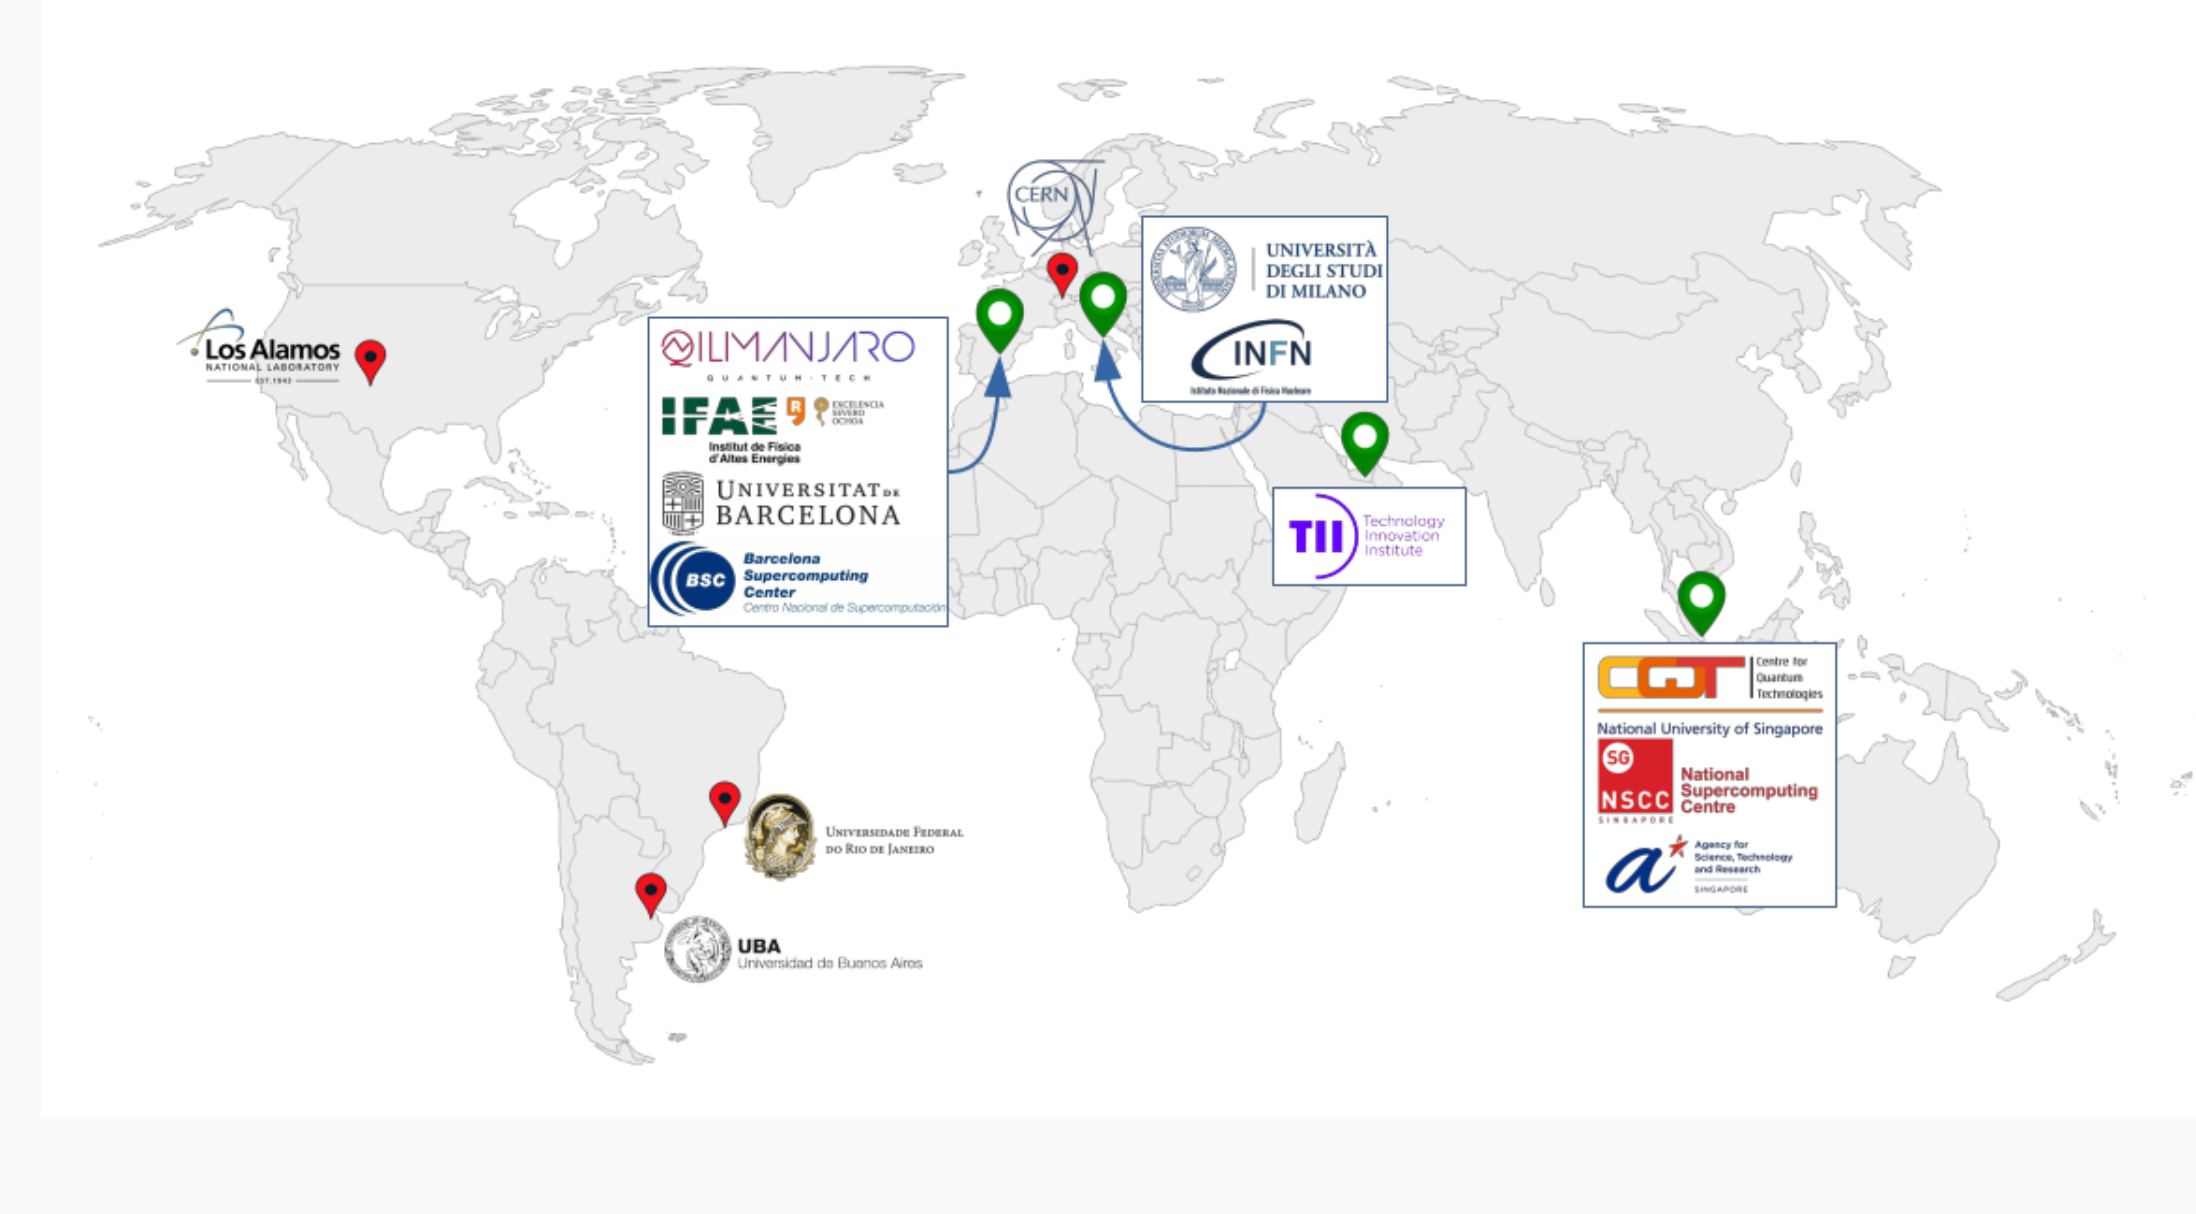
\includegraphics[width=\textwidth]{figures/map.png}
    \end{figure}
    % \begin{columns}
    %     \begin{column}[0.5 \textwidth]
        \begin{table}
            \centering
            \begin{tabular}{lcccc}
                \toprule
                \textbf{Institute} & TII & CQT & INFN & Qilimajiaro\\
                \midrule
                \textbf{Quantum Hardware} & 5 qubits & 10 qubits & 1 qubit & 2 qubits \\
                \bottomrule
            \end{tabular}
            % \caption{Versions of Qibo and its dependencies used in the benchmarks.}
            \label{tab:qibo_versions}
            \end{table}
        % \begin{multicols}{2}
        %     \begin{itemize}
        %         \item Chips with 1 and 5 qubits at TII
        %         \item Chips with 1 and 2 qubits at Qilimanjaro
        %         \item Chip with 1 qubit in Italy (soon)
        %         \item Chips with up to 10 qubits at CQT
        %     \end{itemize}
        % \end{multicols}
    %     \end{column}
    %     \begin{column}[0.5 \textwidth]
    %         test
    %     \end{column}
    % \end{columns}
\end{frame}

\begin{frame}{Challenge}
    \begin{figure}
        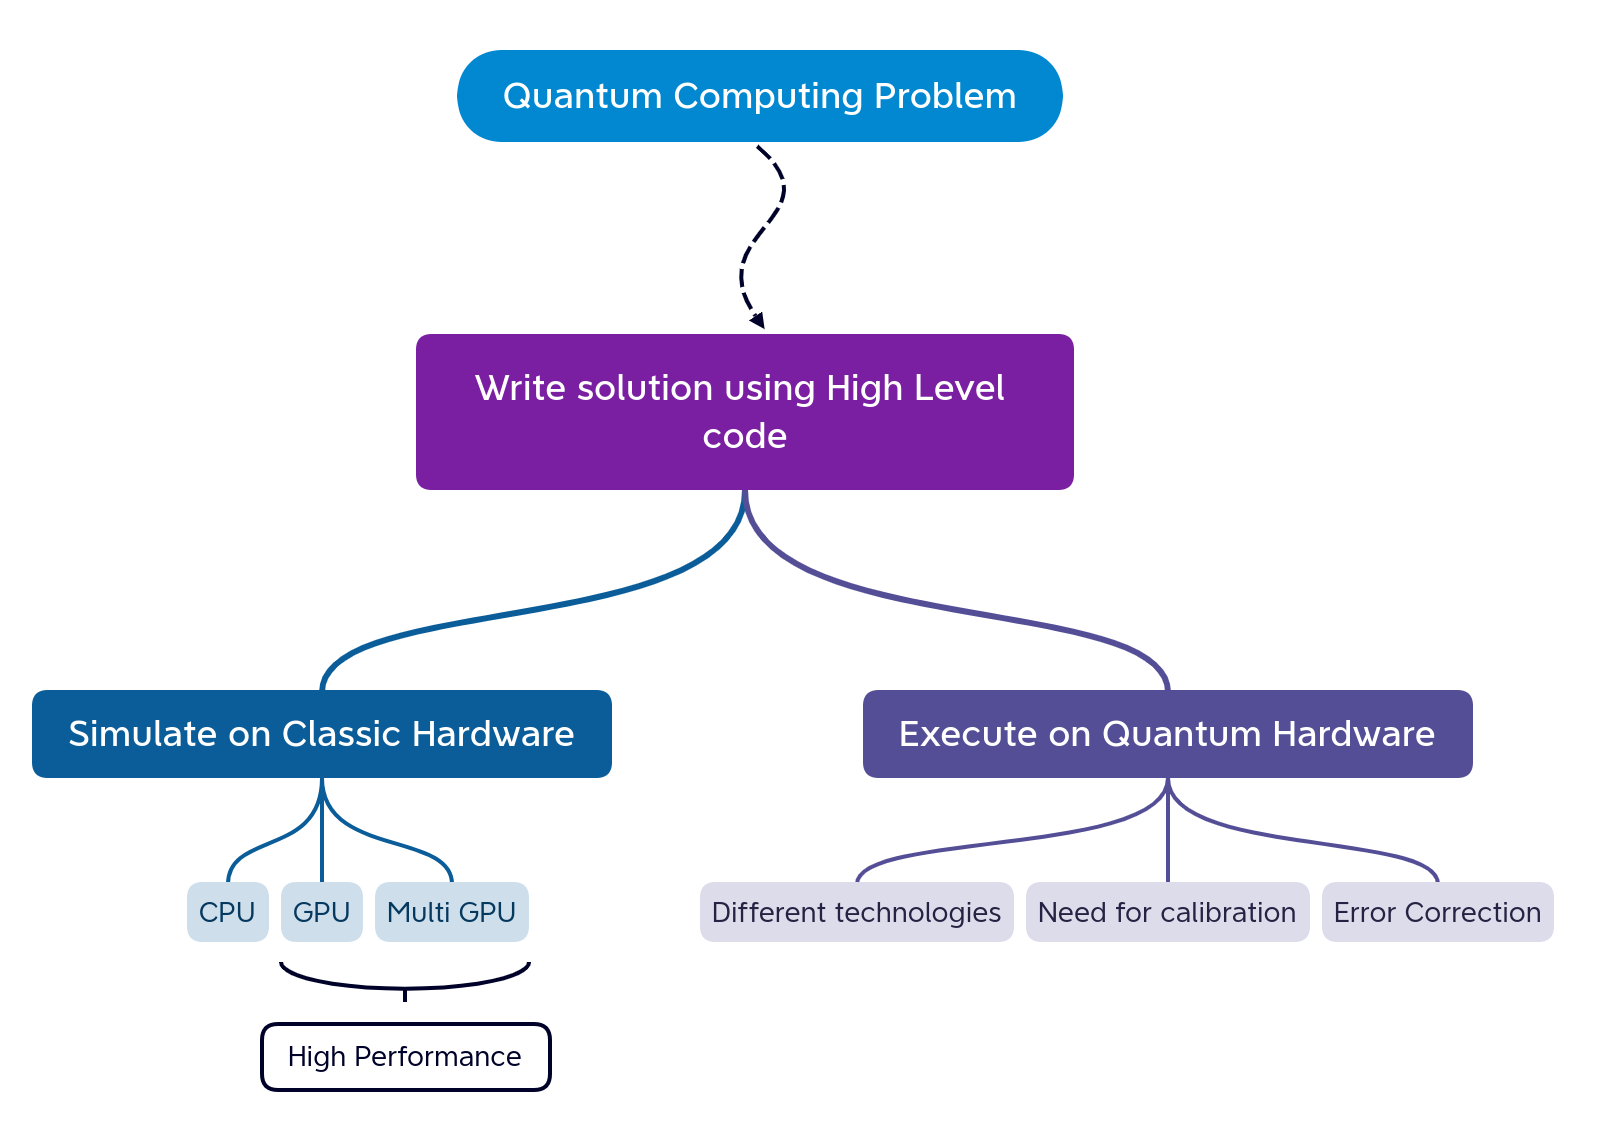
\includegraphics[width=\textwidth]{figures/intro.png}
    \end{figure}
    \vspace{-0.5cm}

    \centering
    \emph{Is to possible to create from scratch a framework for all of this?}
\end{frame}


% \begin{frame}{User problem}
    
    
% \end{frame}



\section{Introducing Qibo}

\begin{frame}{Qibo}
    Qibo is an \textbf{open-source} full stack API for quantum simulation and quantum hardware control and calibration.
    \begin{figure}
        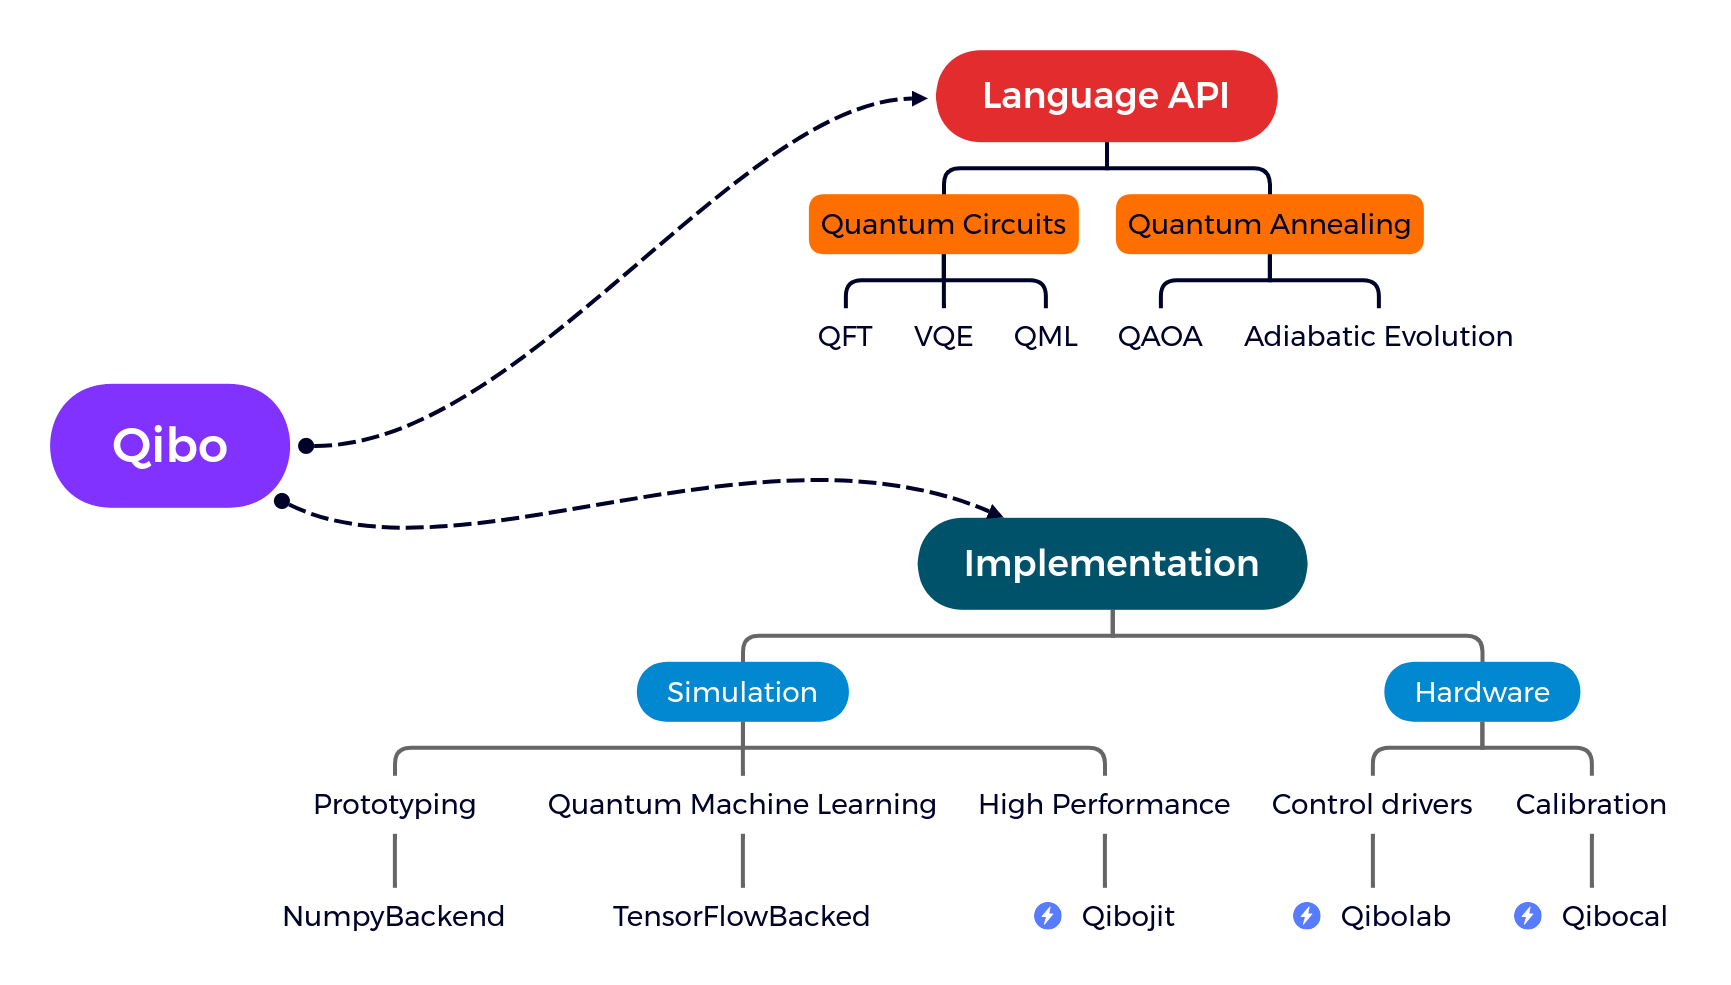
\includegraphics[width= \textwidth]{figures/Qibo.png}
    \end{figure}
    \vspace{-1cm}
\begin{center}
    \url{https://github.com/qiboteam/qibo}
\end{center}
\end{frame}

% \begin{frame}{A modular framework for quantum computing}
%     \begin{figure}
%         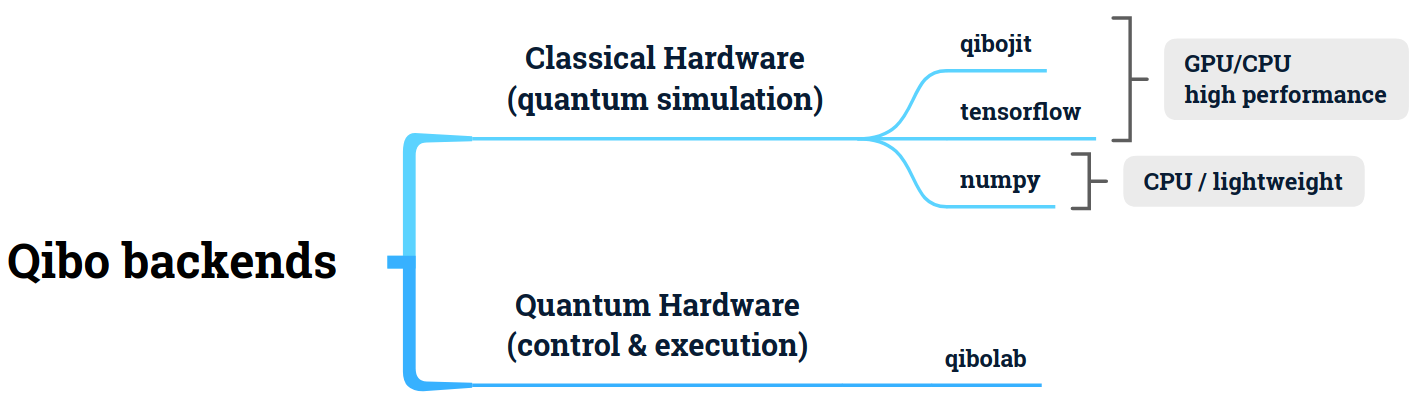
\includegraphics[width= \textwidth]{figures/backends.png}
%     \end{figure}
% \end{frame}

\begin{frame}{Introducing Qibojit}
    Matrix multiplication to simulate circuits:

    \begin{equation*}\label{eq:gateapplication}
        \psi'(\sigma_1, \ldots, \sigma_n) = \sum _{\boldsymbol{\tau'}} G(\boldsymbol{\tau}, \boldsymbol{\tau'})\psi(\sigma_1,\ldots,\boldsymbol{\tau'},\ldots,\sigma_n) \ .
    \end{equation*}

    
    
    { \color{red} \faClose}  Number of operations scales { \color{red} exponentially} with the number of qubits!
   
    We need more sophisticated backends to perform simulation:
    \begin{itemize}
        \item[{ \color{red} \faClose}] \texttt{NumpyBackend} : { \color{blue} Numpy} tensors and primitives
        \item[{ \color{red} \faClose}] \texttt{TensorFlowBackend} : { \color{orange} Tensorflow} tensors and primitives
        \item[{ \color{green} \faCheck}] \texttt{QibojitBackend} : Just-In-time
        \item[]     \begin{itemize}
            \item[\faCode] CPU : { \color{blue} Numpy} tensor + custom operations with {\color{cyan} Numba JIT}
            \item[\faCode] GPU(S) : {\color{teal} Cupy} tensors + custom operations using
            \begin{itemize}
                \item  {\color{teal} Cupy JIT} Raw kernels
                \item  {\color{green} NVIDIA cuQuantum}  API
            \end{itemize} 
        \end{itemize}
    \end{itemize}

    Paper published on Quantum: \url{https://quantum-journal.org/papers/q-2022-09-22-814/}

    
\end{frame}

\begin{frame}[fragile]{Qibojit - Example}

    \begin{columns}
        \begin{column}{0.7\textwidth}
            \hspace{1cm}
            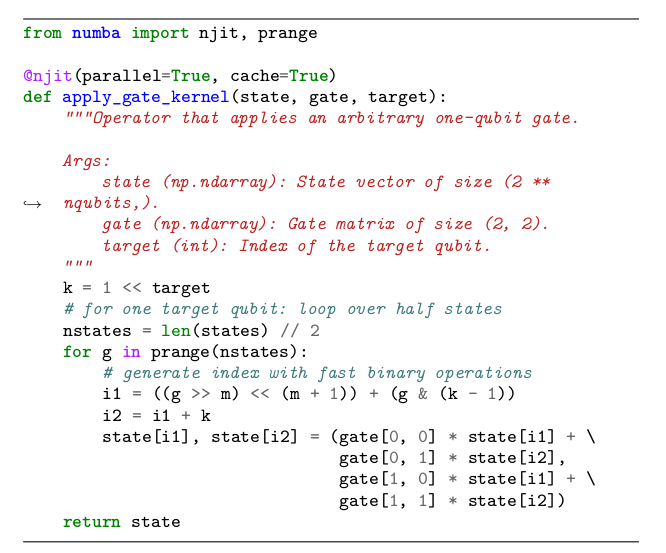
\includegraphics[width = 0.8\textwidth]{figures/circuit.png}
        \end{column}

        \begin{column}{0.6\textwidth}
            To further speed up:
            \begin{itemize}
                \item \emph{in-place updates}
                \item exploit sparsity of matrices
                \item specialized operators for:
                \begin{itemize}
                    \item single qubit gate: X, Y Z
                    \item two qubit gates: SWAP
                \end{itemize}
            \end{itemize}
        \end{column}
    \end{columns}

    
\end{frame}

% \begin{frame}{Benchmarks}
%     \begin{figure}
%         % 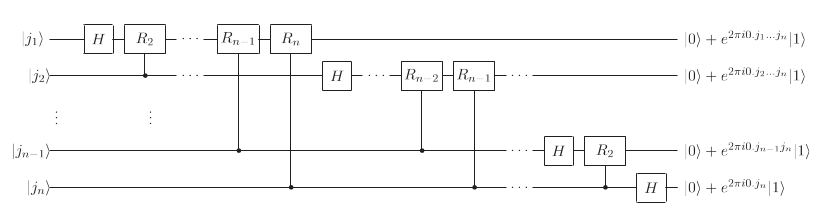
\includegraphics[width=0.8 \textwidth]{figures/qft.png}
%         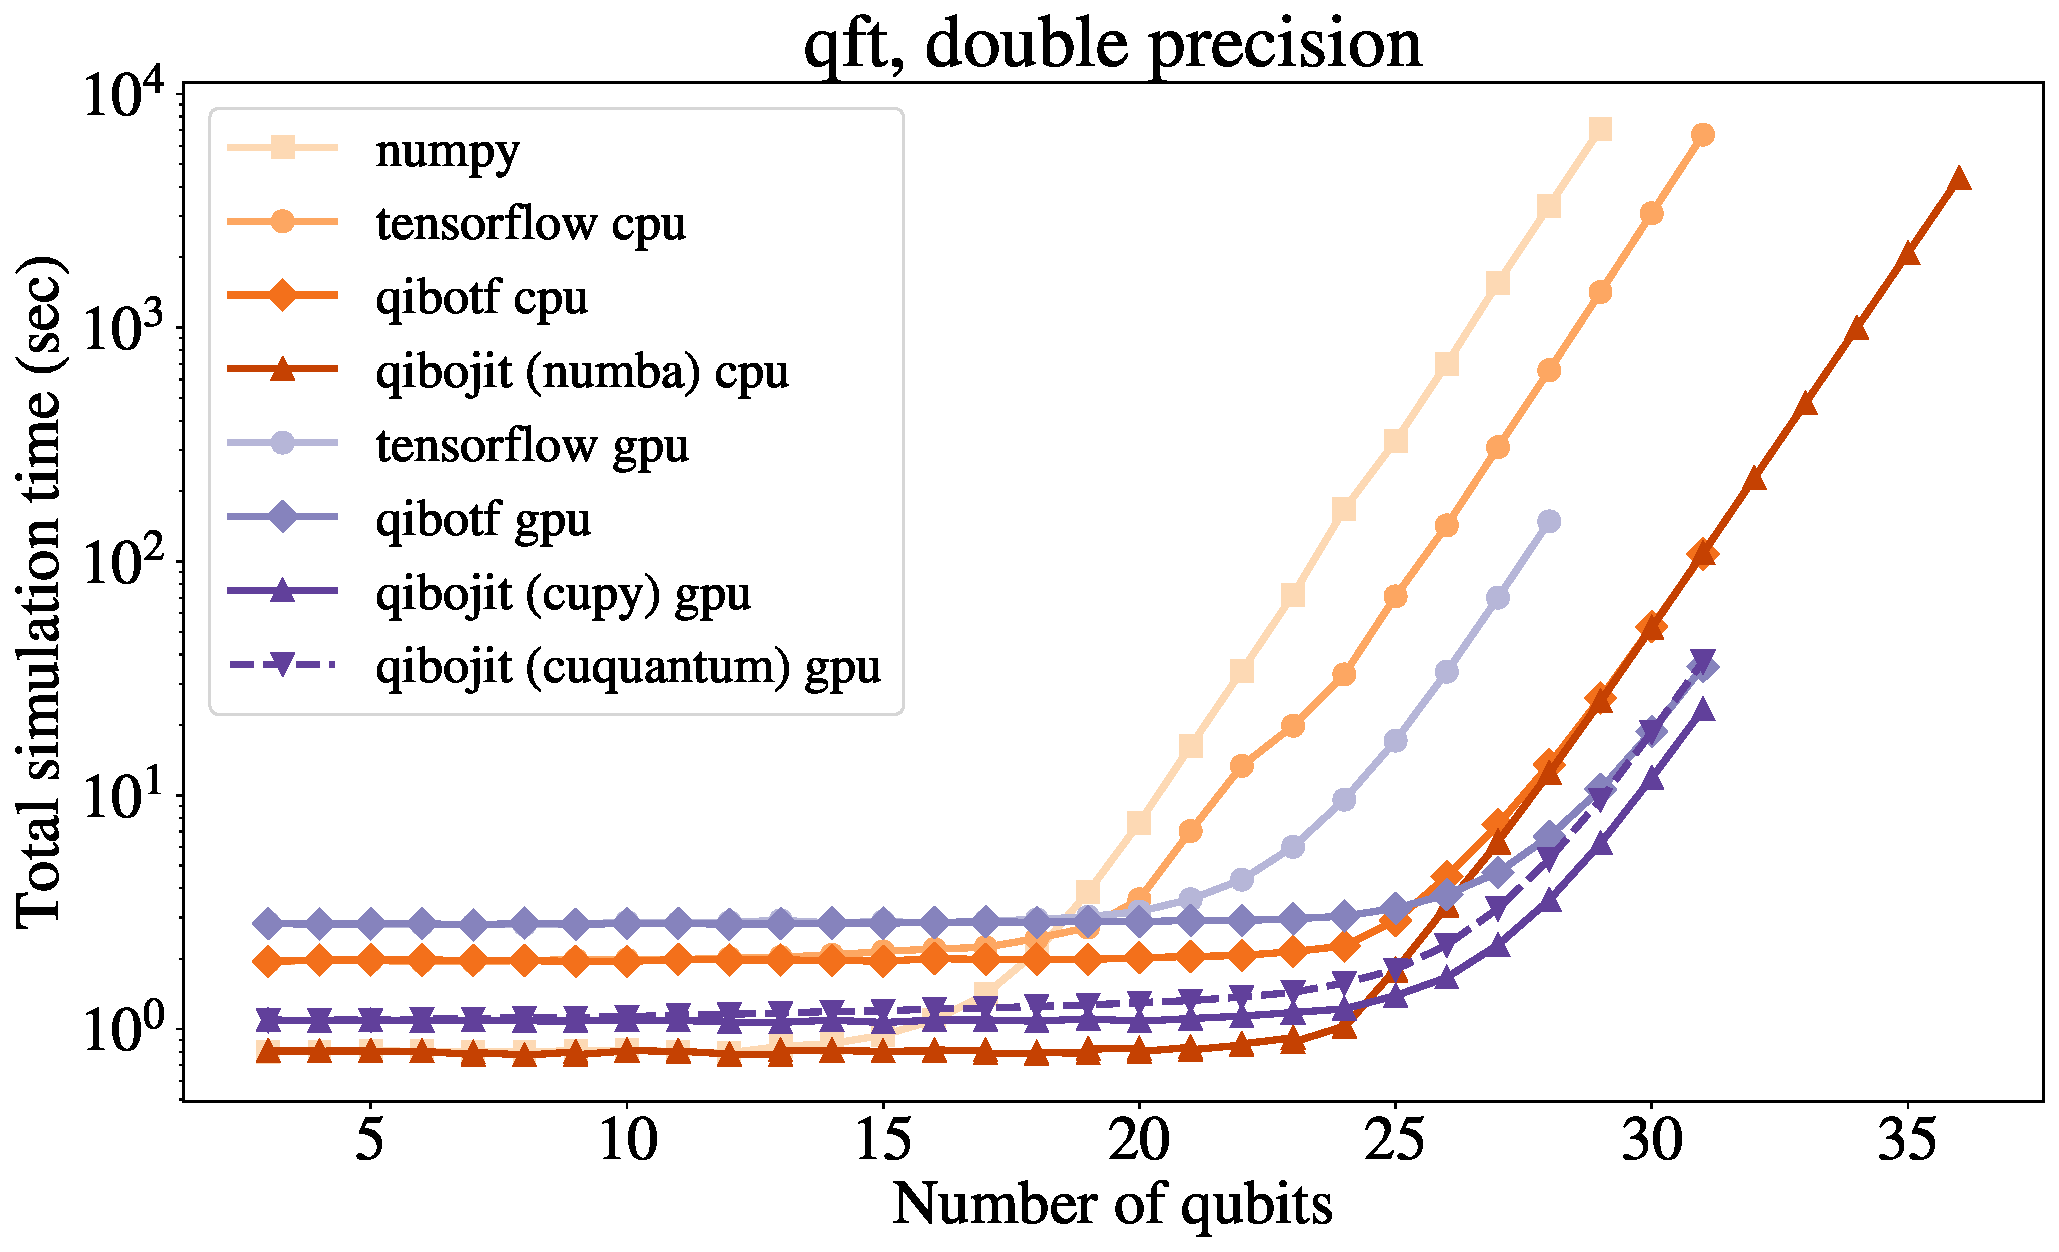
\includegraphics[width=0.8 \textwidth]{figures/qibo_scaling_qft_total_simulation_time_double.pdf} 
%     \end{figure}
%     Benchmark library: \url{https://github.com/qiboteam/qibojit-benchmarks}
% \end{frame}

% \begin{frame}{Benchmarks}
%     \begin{columns}
%         \begin{column}{0.8 \textwidth}

%             % \begin{figure}[ht]
%             %     \fbox{\begin{minipage}[t]{0.8 \textwidth}
%             %       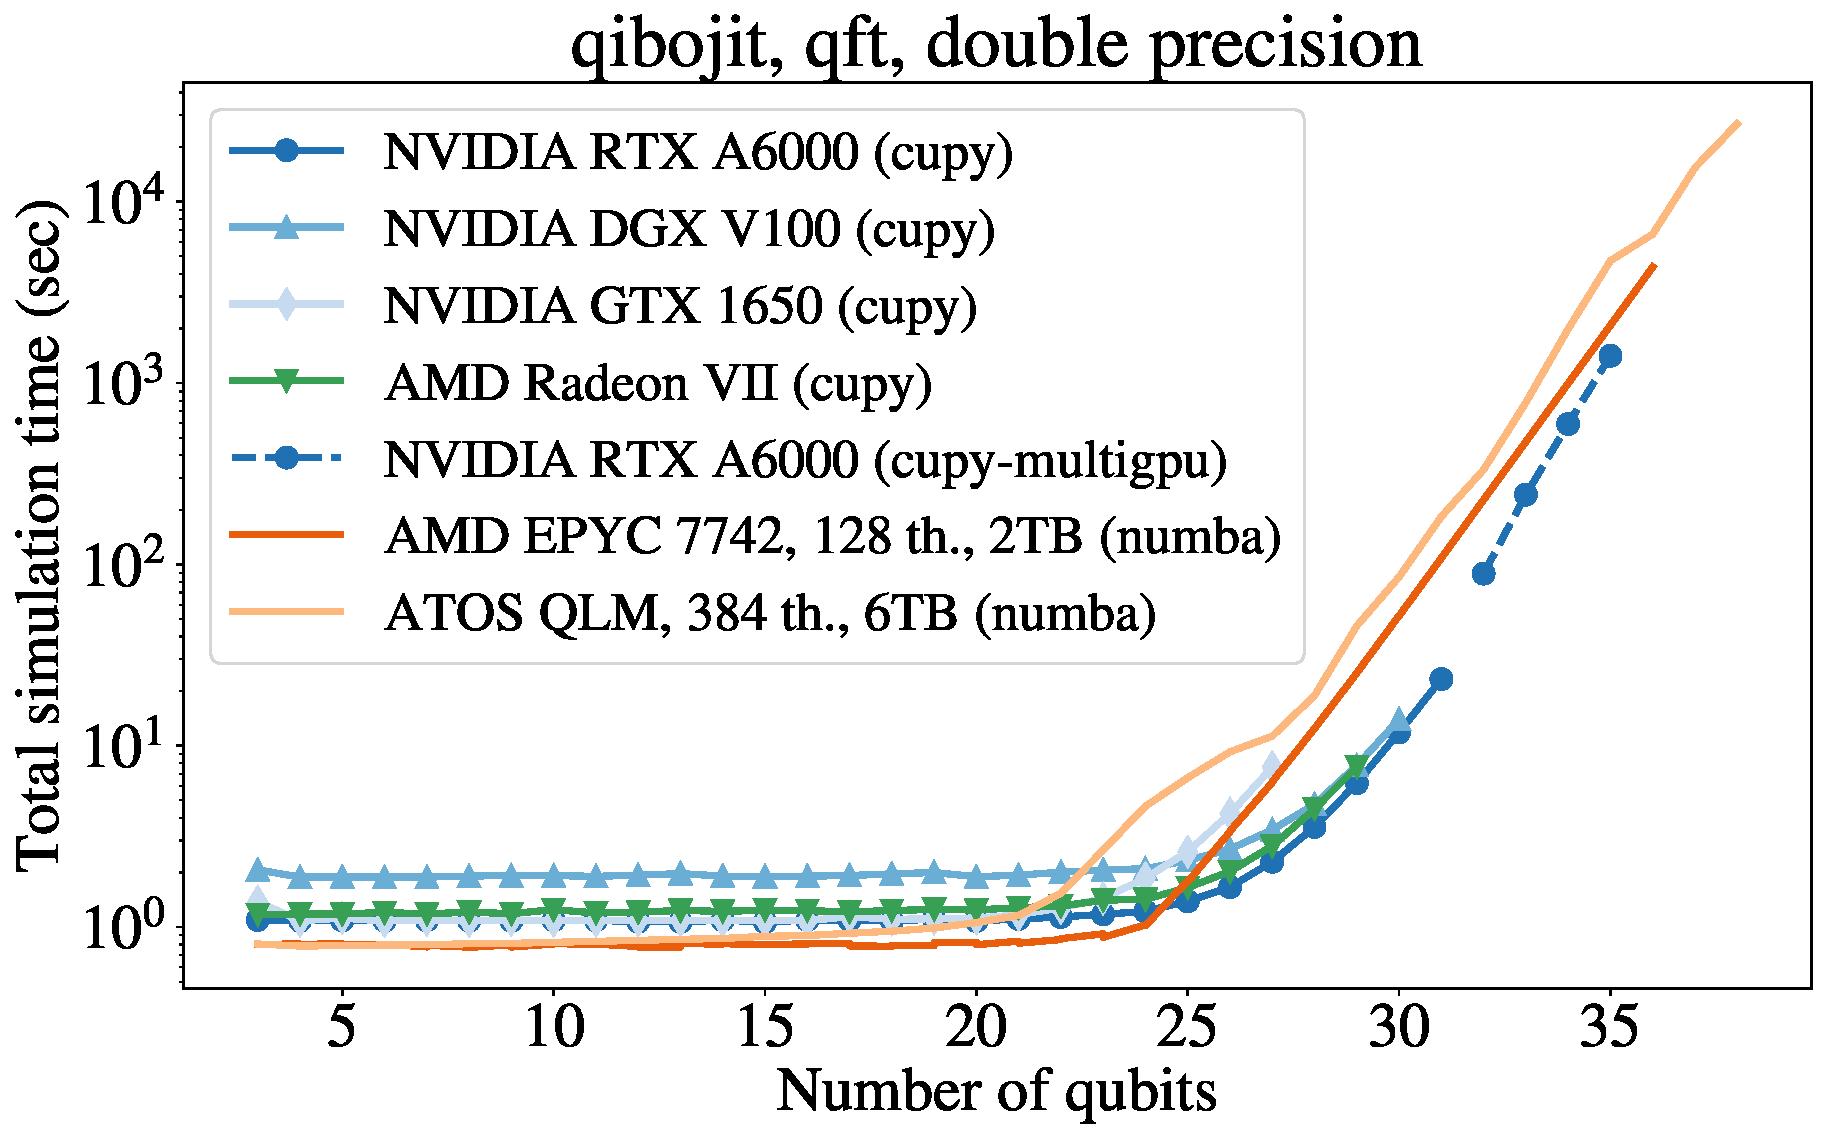
\includegraphics[width=0.8 \textwidth]{figures/devices_qft_total_simulation_time_double.pdf}
%             %     \end{minipage}}
%             %     \hfill
%             %     \fbox{\begin{minipage}[t]{0.8 \textwidth}
%             %       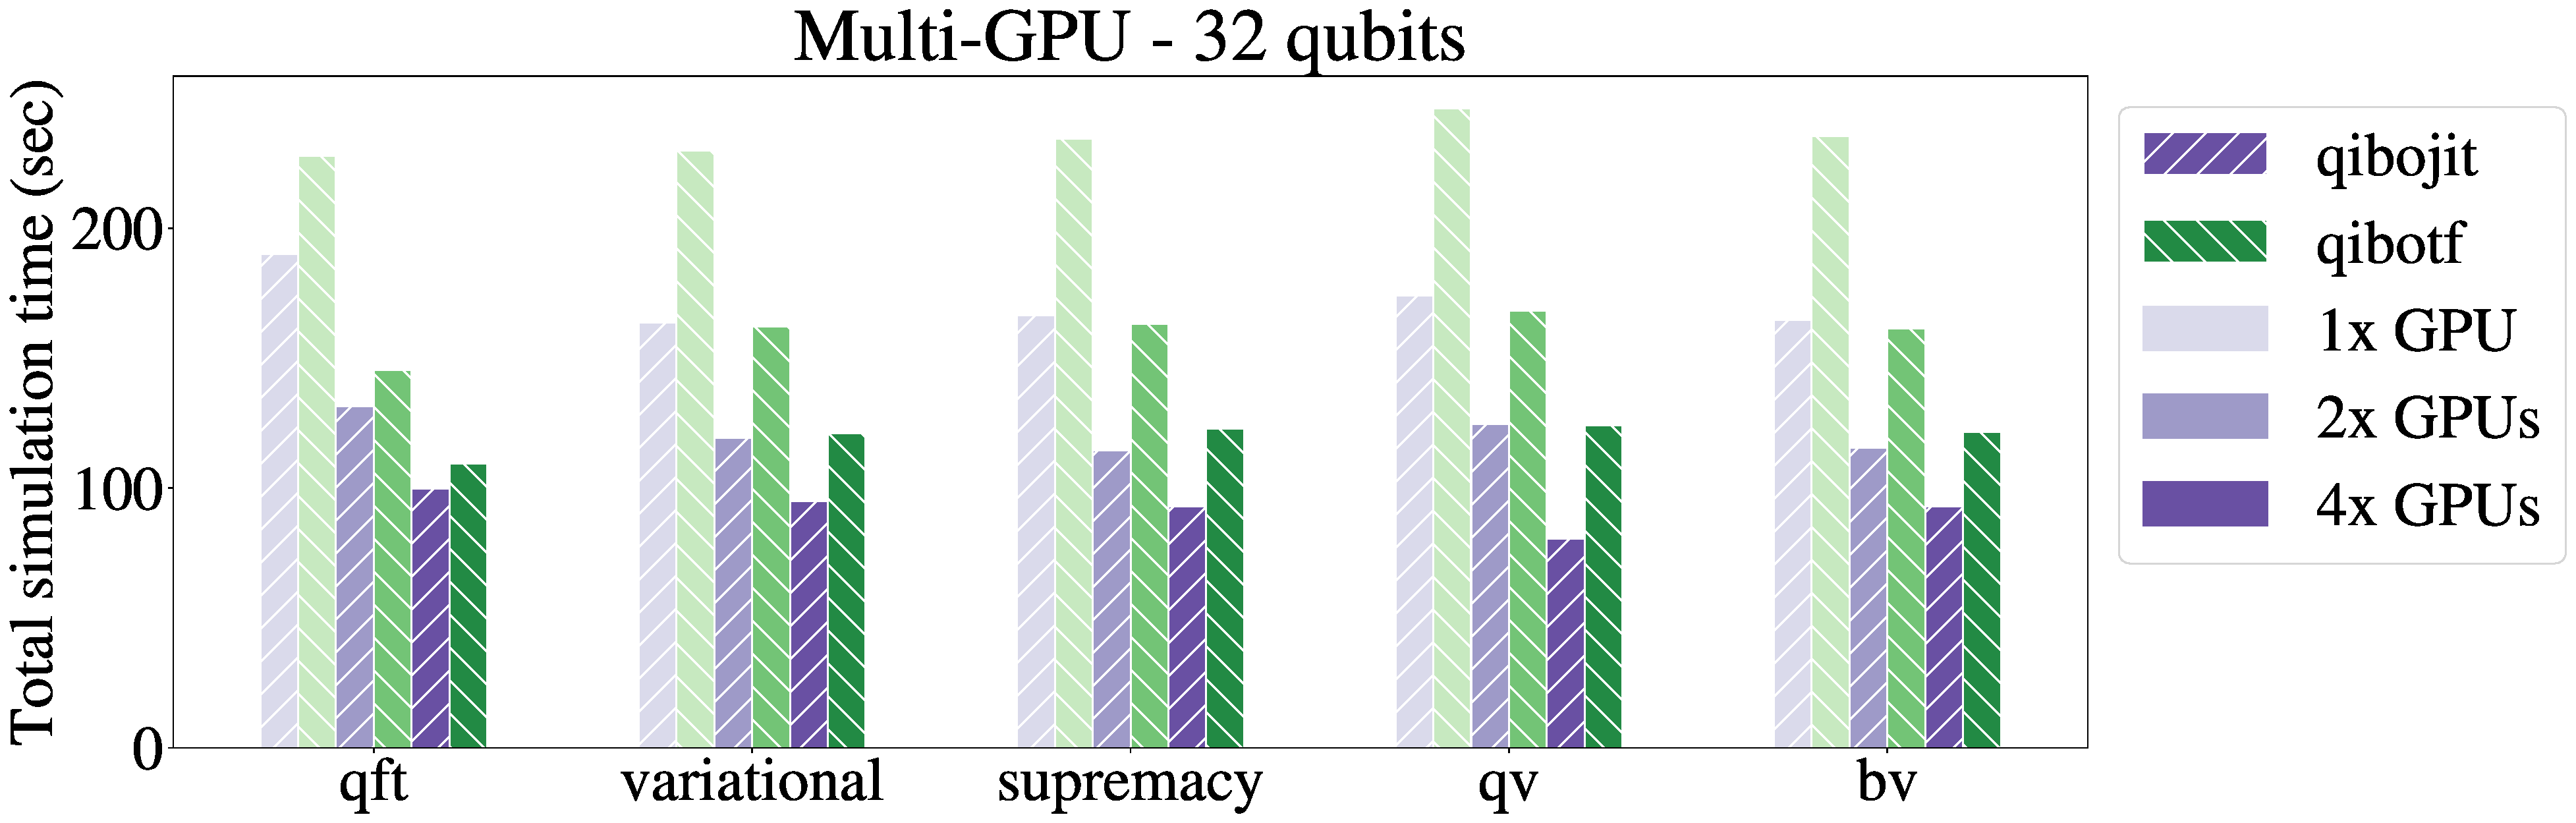
\includegraphics[width=0.8 \textwidth]{figures/multigpu_32qubits_total_simulation_time_double.pdf}
%             %     \end{minipage}}
%             %   \end{figure}
%             \begin{figure}
%             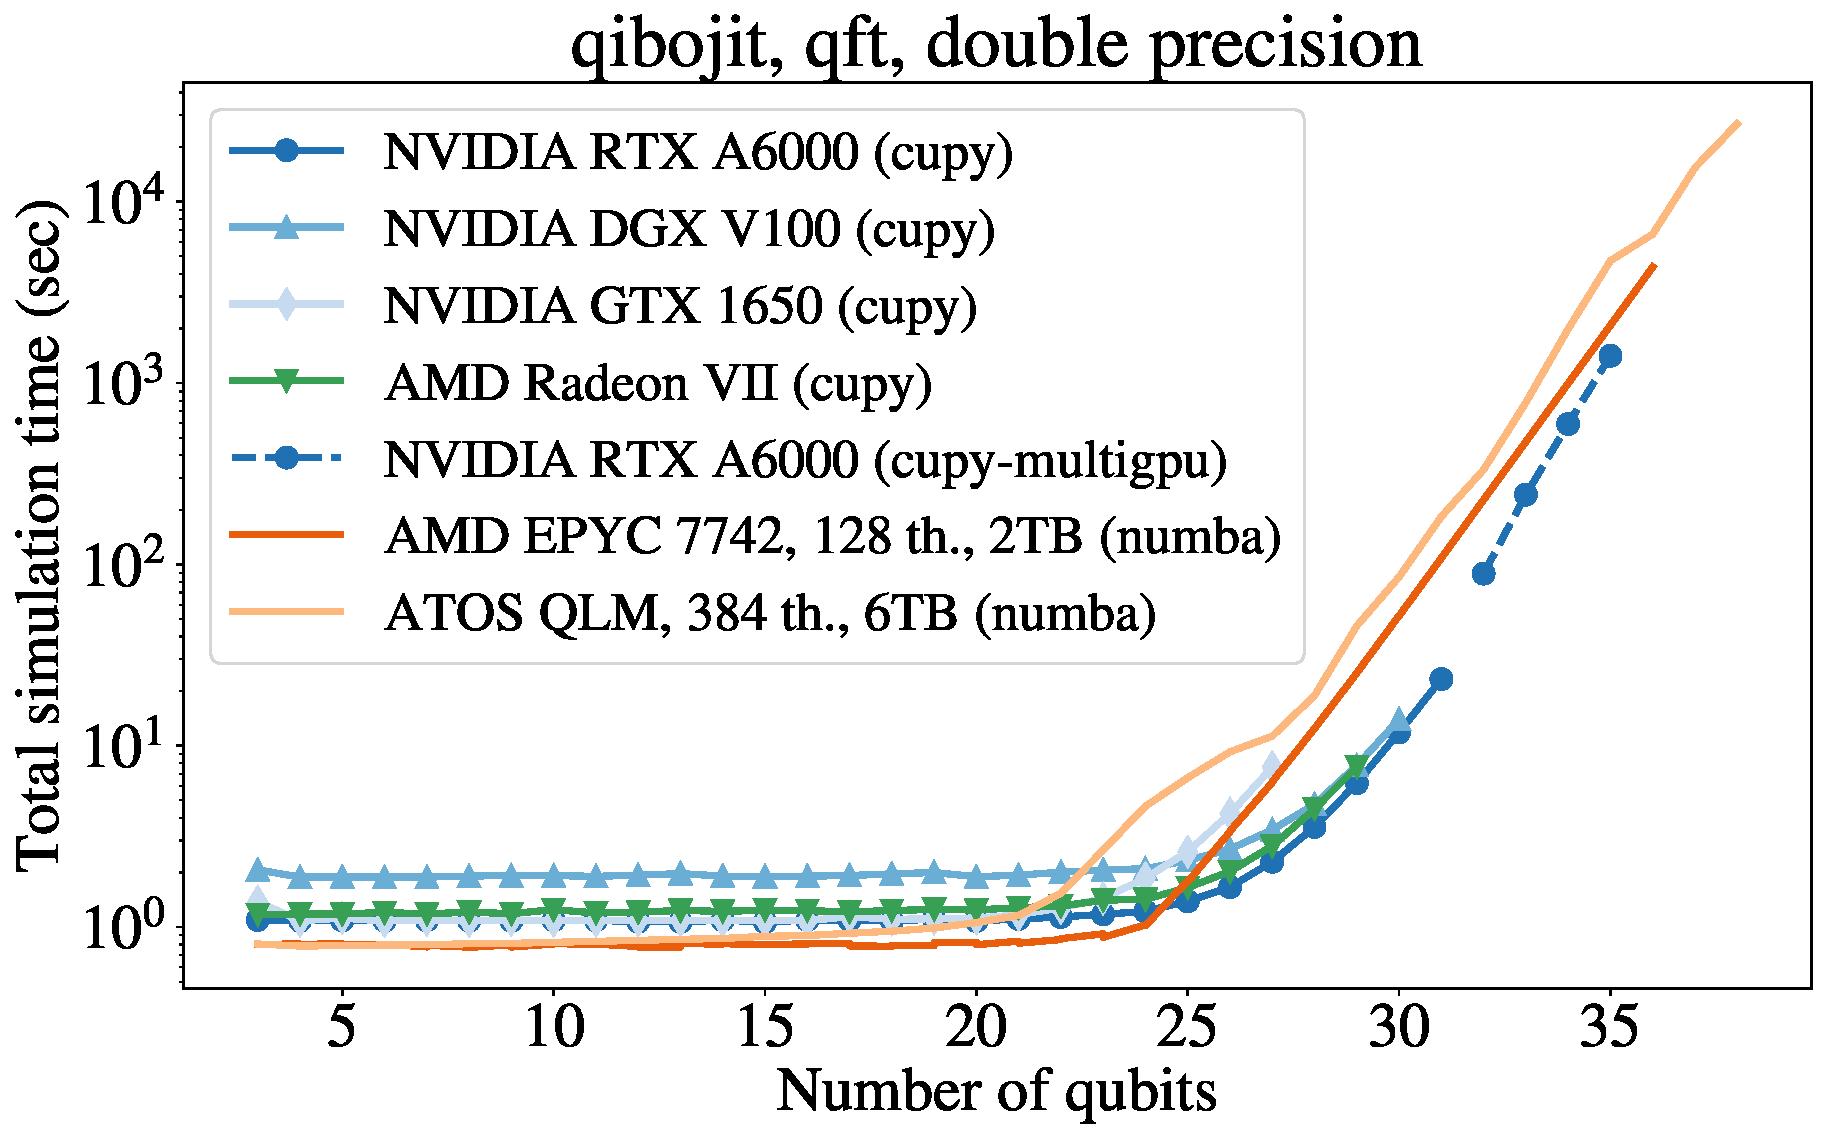
\includegraphics[width=0.8 \textwidth]{figures/devices_qft_total_simulation_time_double.pdf}
%             \hspace{0.5cm}

%             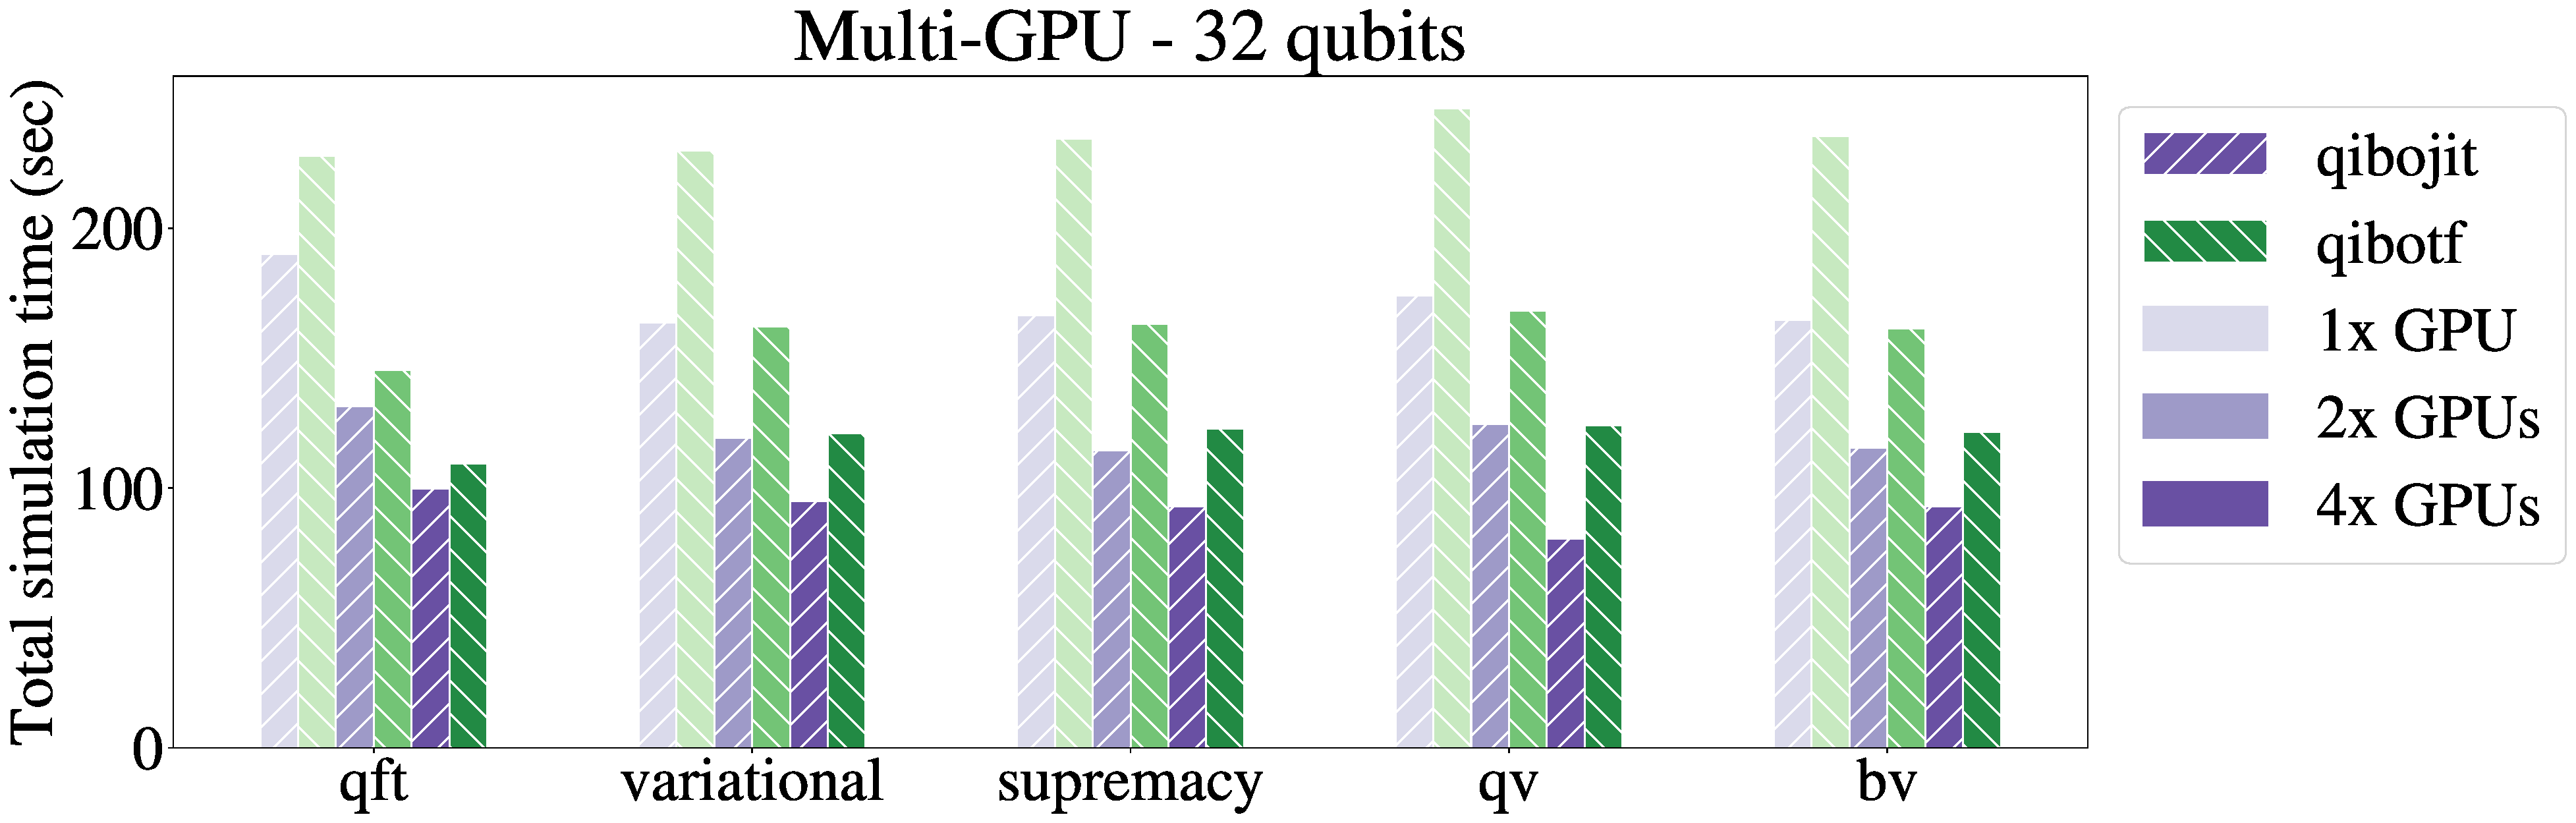
\includegraphics[width=0.8 \textwidth]{figures/multigpu_32qubits_total_simulation_time_double.pdf}
%             \end{figure}
%         \end{column}
%         \hspace{-1cm}
%         \begin{column}{0.4 \textwidth}
%             \vspace{-1cm}

%             Qibojit features
%             \begin{itemize}
%                 \item Support for CPU, GPU and multi-GPU
%                 \item NVIDIA and AMD (ROCm) GPUs
%                 \item Reduced memory footprint
%             \end{itemize}
%         \end{column}
%     \end{columns}
%     Benchmark library: \url{https://github.com/qiboteam/qibojit-benchmarks}
    
% \end{frame}


\begin{frame}{How does Qibo perform against the other libraries?}
    \begin{figure}
        \centering
        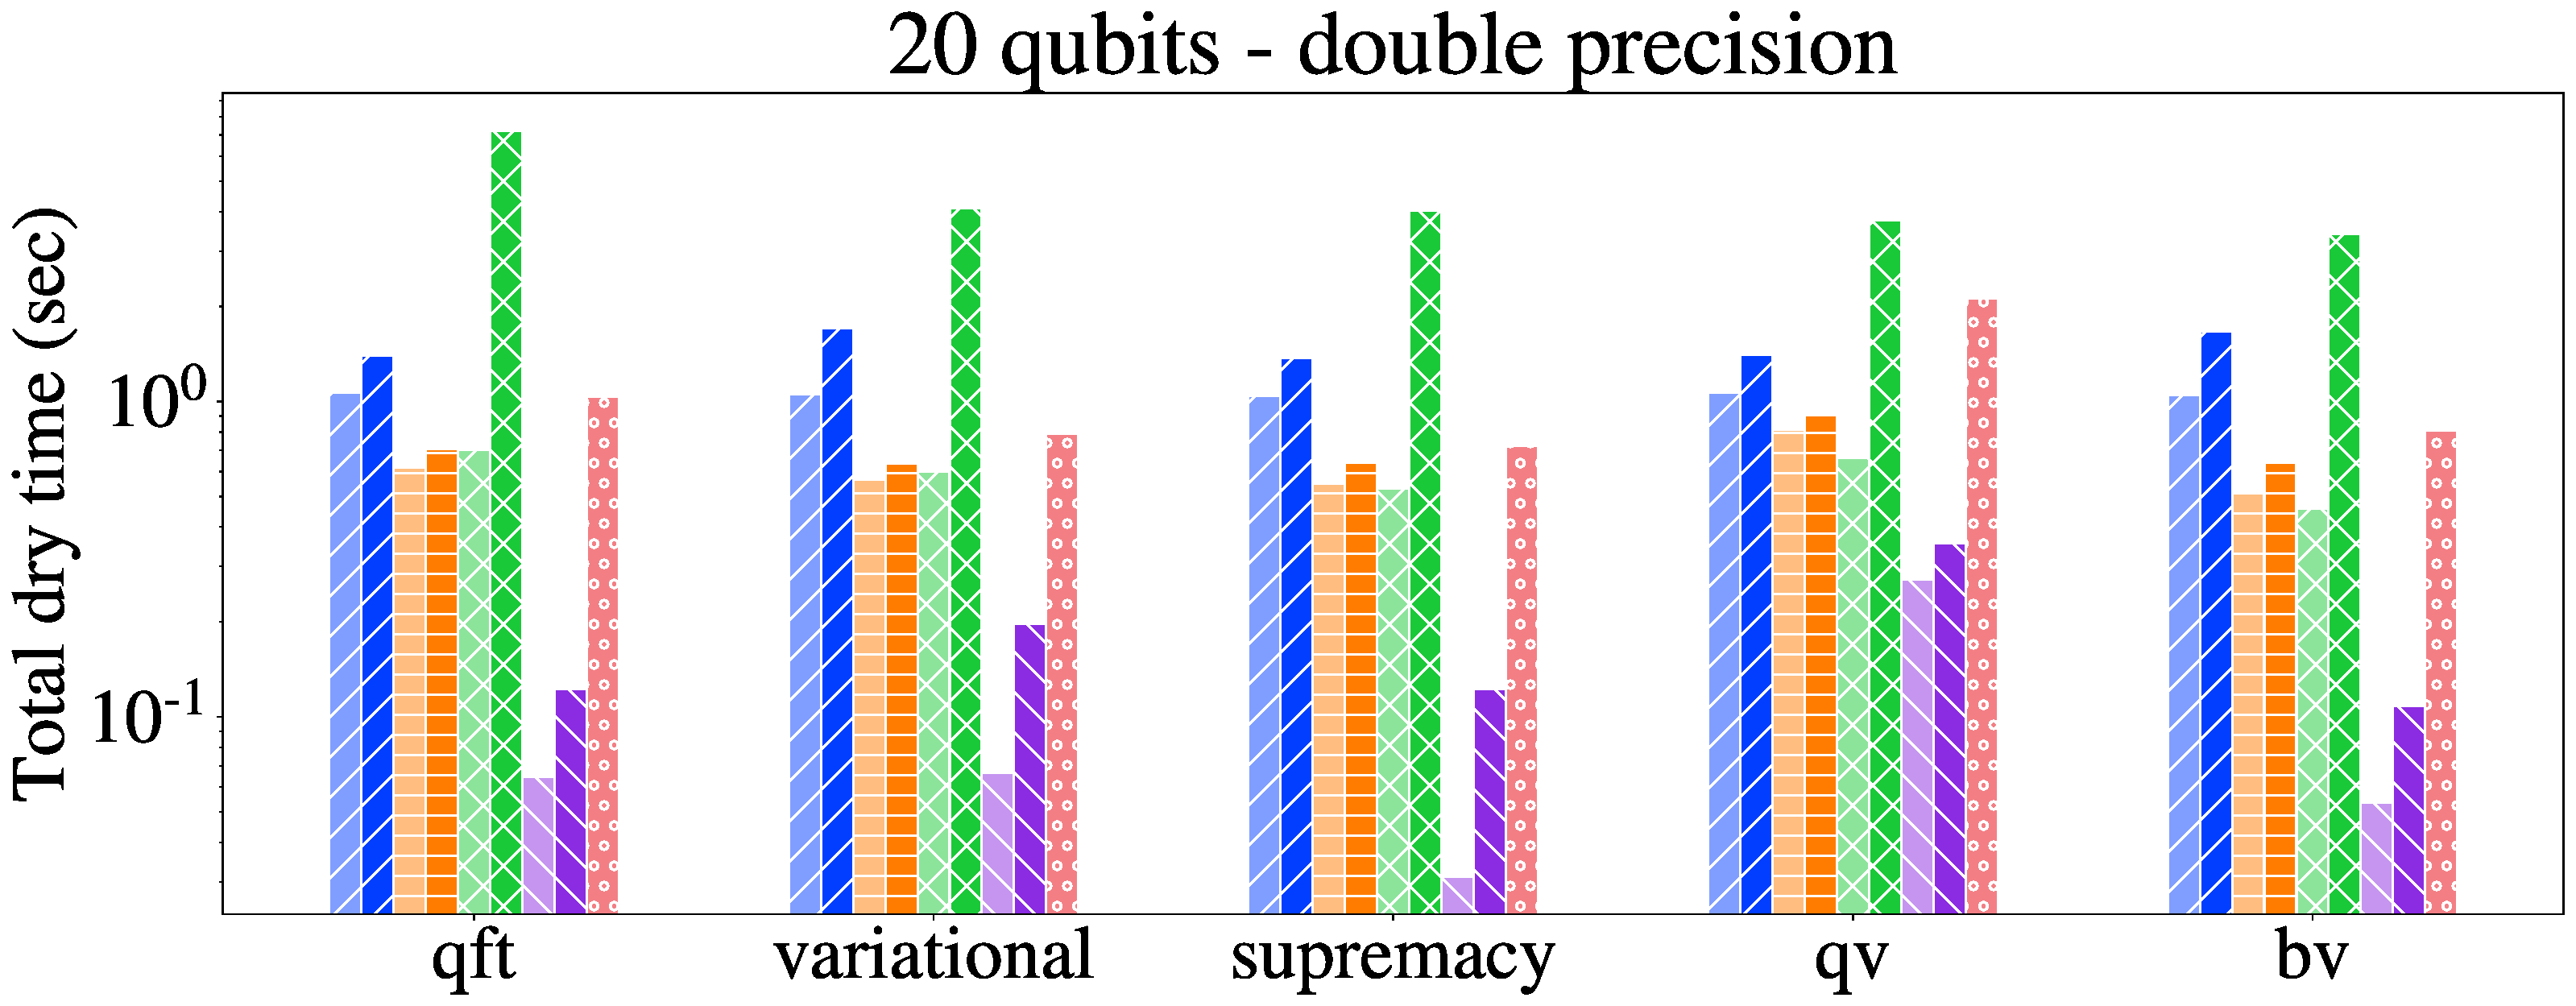
\includegraphics[height=0.4\textheight]{figures/libraries_double_20qubits_total_dry_time.pdf}
        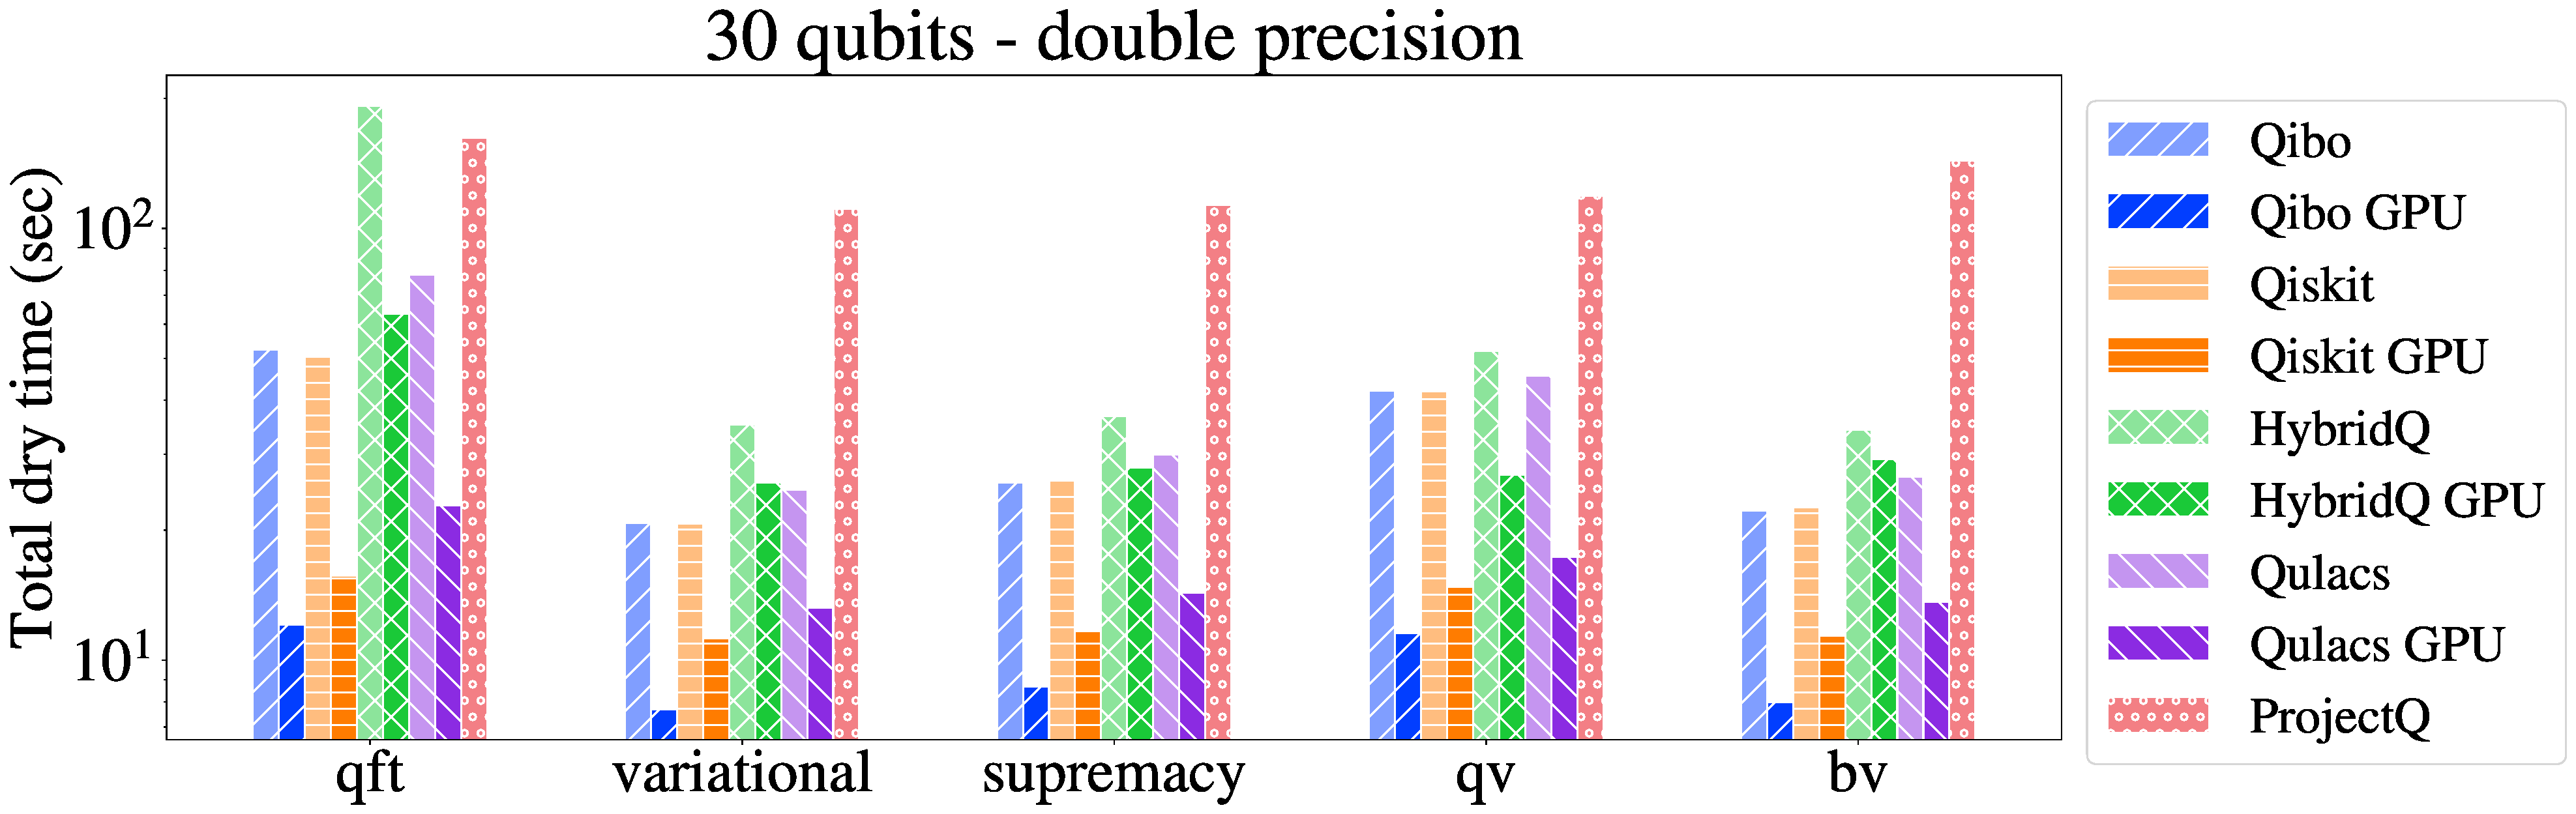
\includegraphics[height=0.31\textheight]{figures/libraries_double_30qubits_total_dry_time.pdf}
    \end{figure}
    Benchmark library: \url{https://github.com/qiboteam/qibojit-benchmarks}
    
\end{frame}

\section{Hardware control using Qibo}

% \begin{frame}{Hardware control}
%     A quantum computer has many components outside the chip...
%     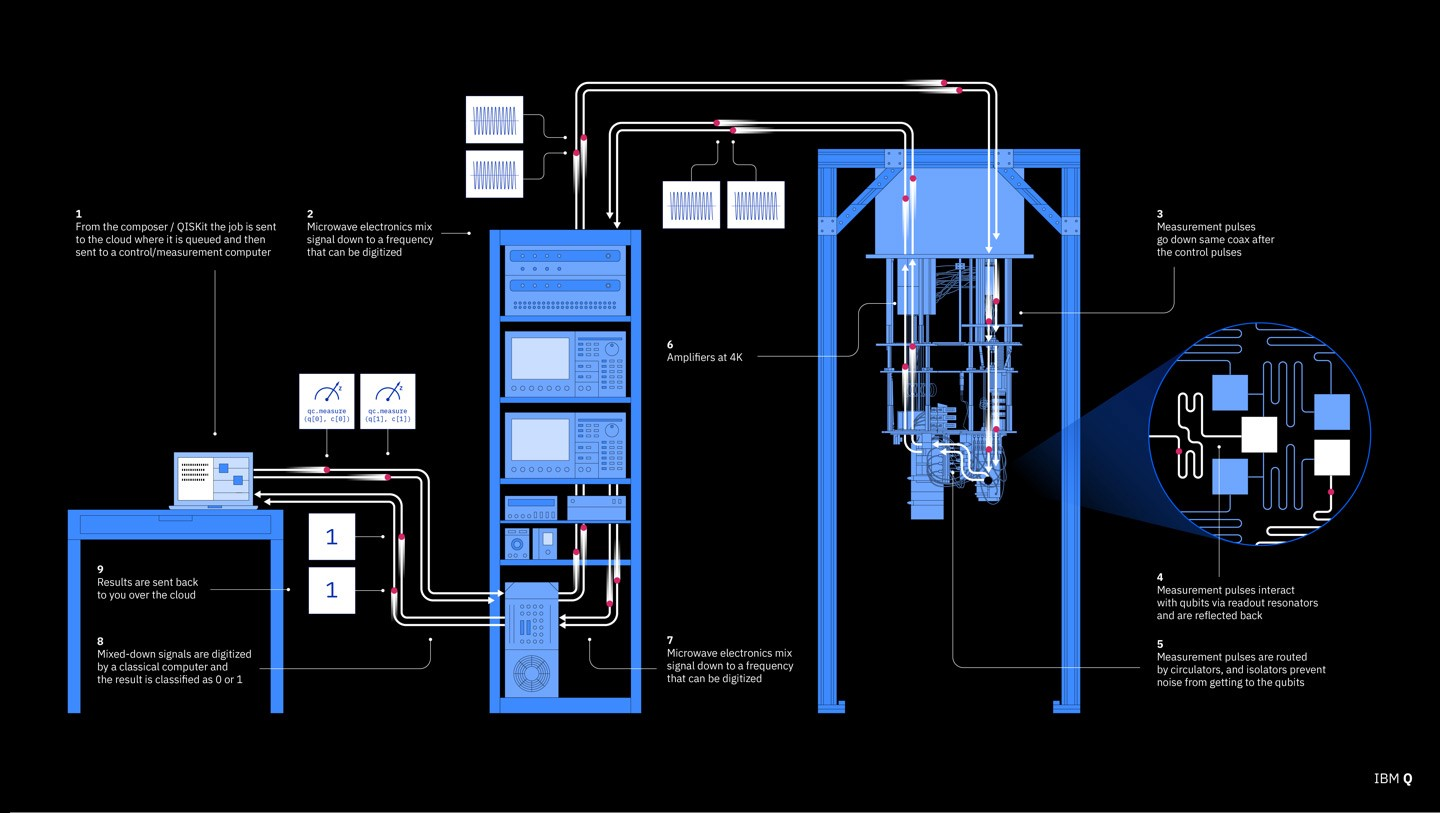
\includegraphics[width = \textwidth]{figures/quantum_computer.jpeg}


    
% \end{frame}

\begin{frame}{Hardware control}
    For superconducting qubits \textbf{gates} are implemented by sending \textbf{pulses}.

    \begin{columns}
        \begin{column}{0.5 \textwidth}
            \begin{figure}
                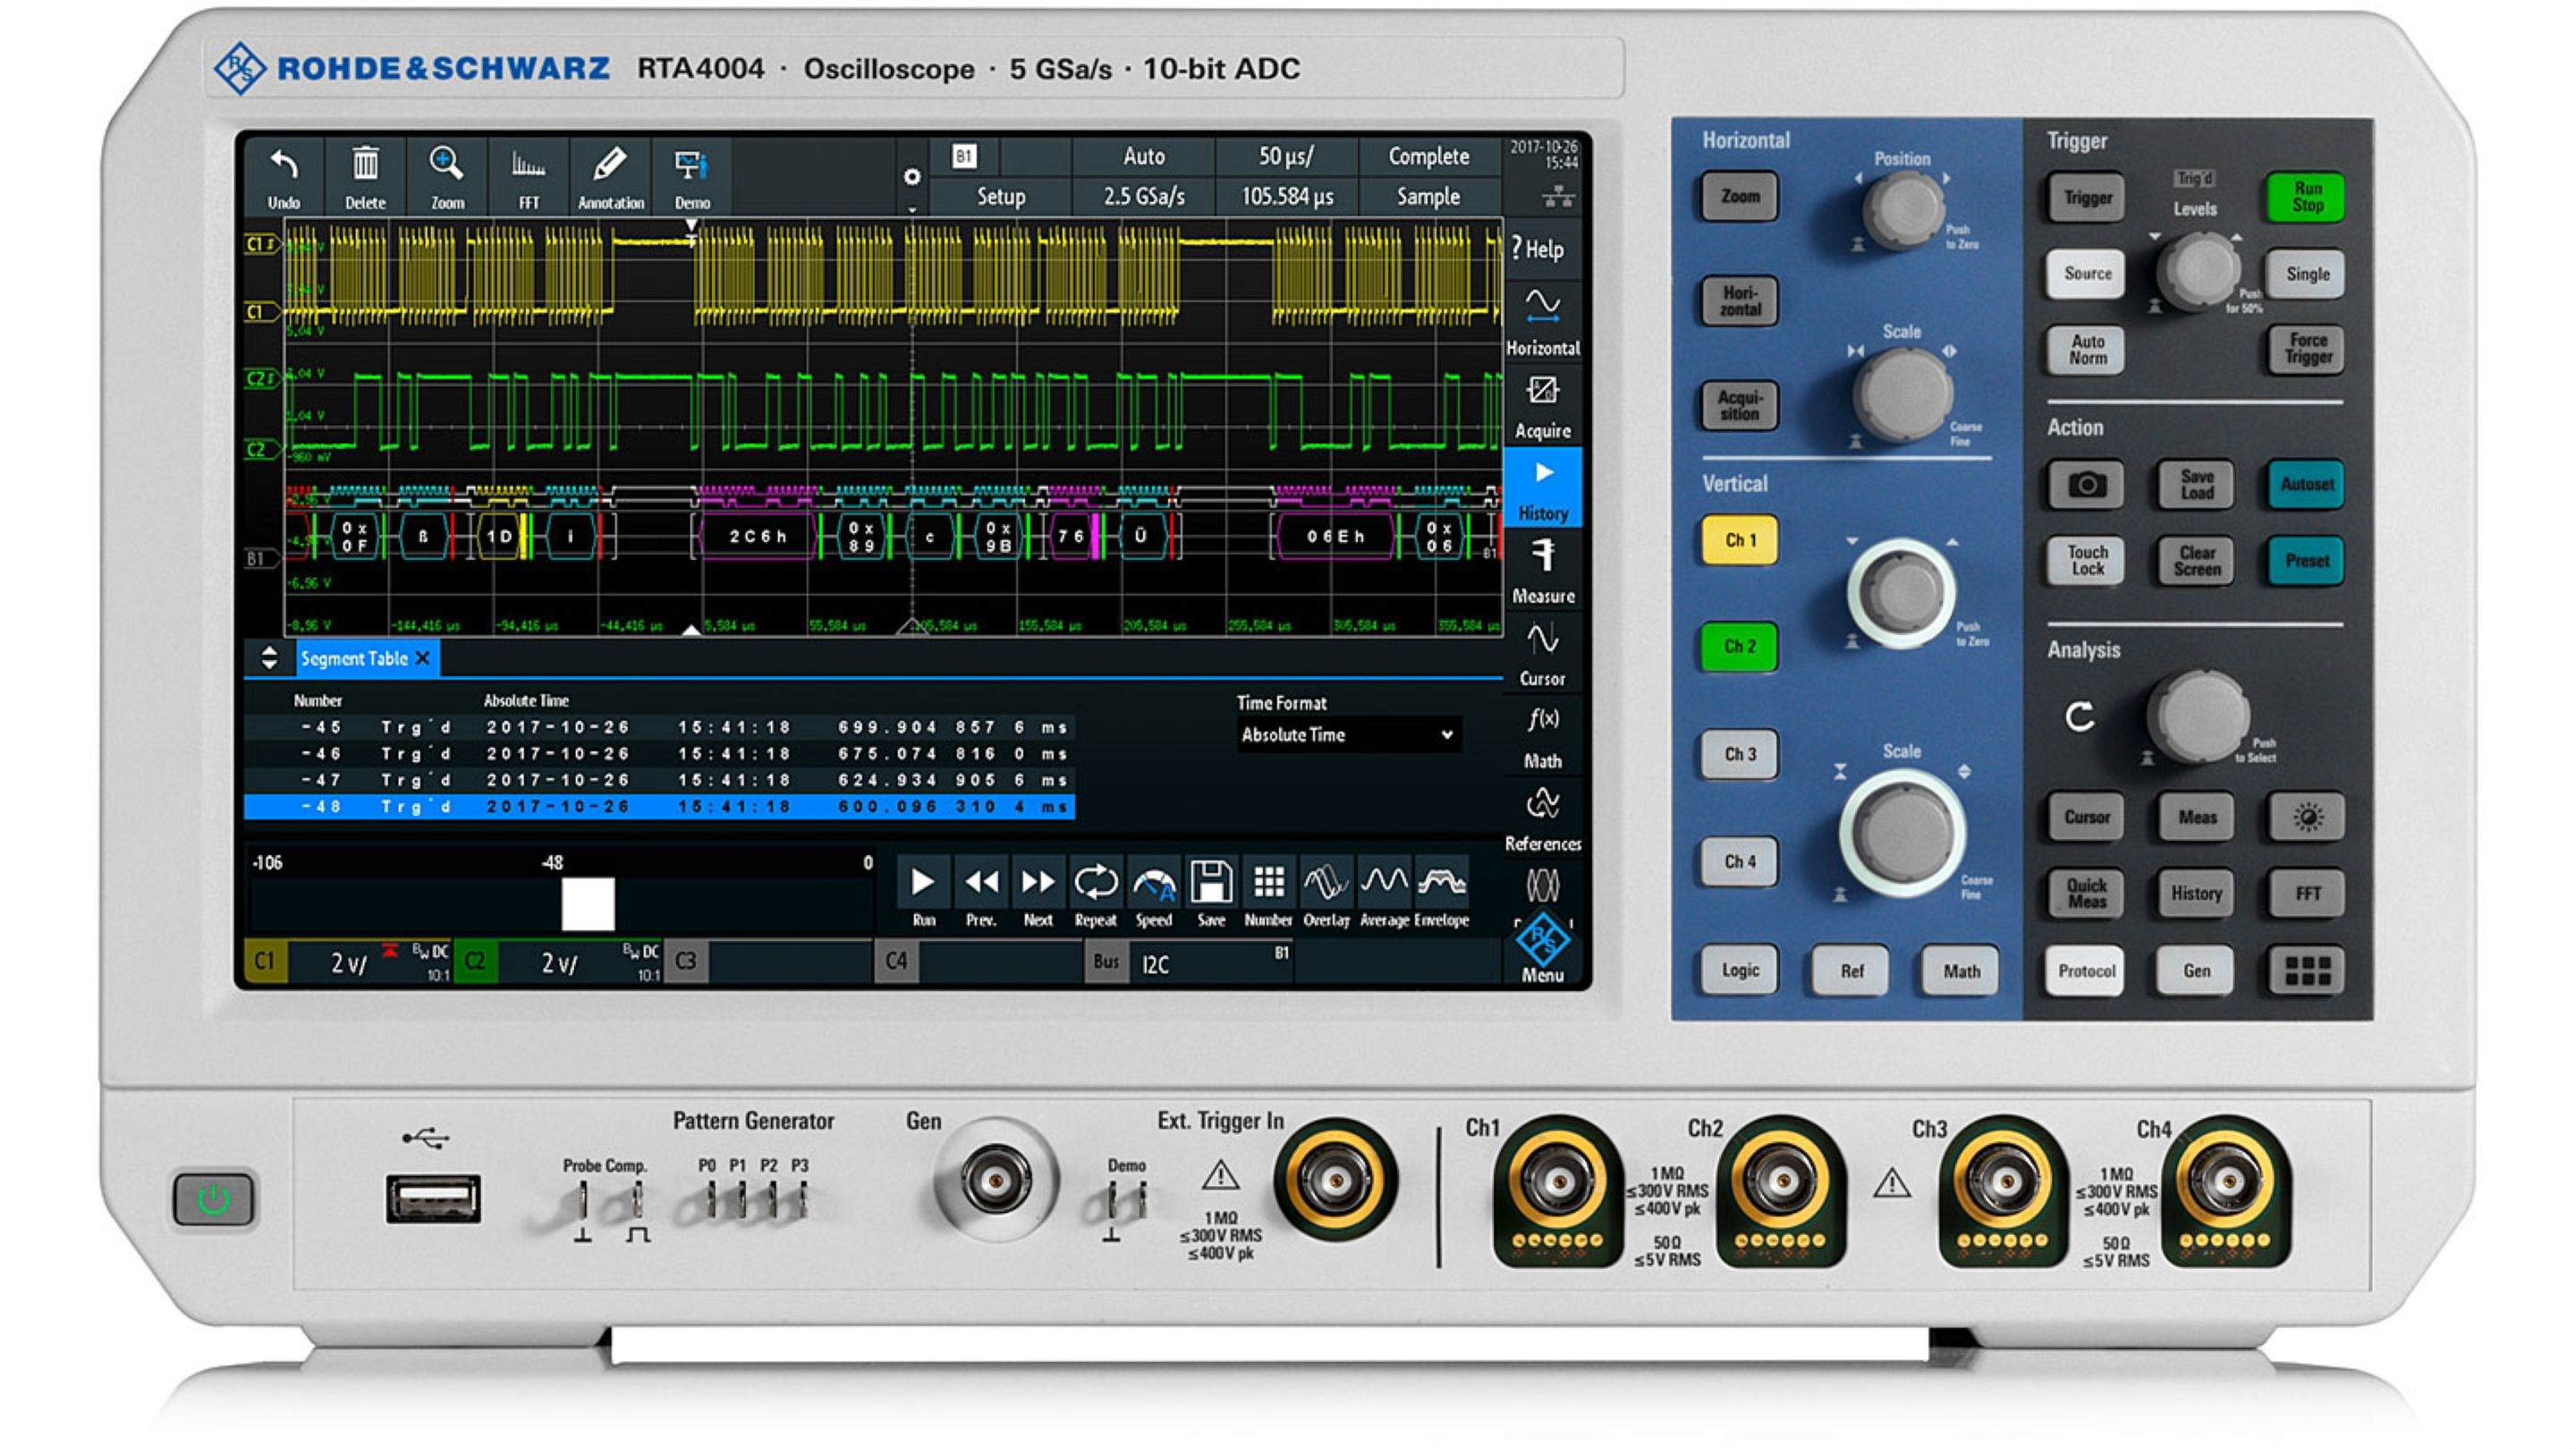
\includegraphics[height = 0.3 \textheight]{figures/rohde.jpg}
                % \caption{Oscilloscope}
            \end{figure}
            
            % \begin{itemize}
            %     \item Wavefunction generators
            %     \item Local oscillators
            %     \item Qblox devices
            %     \item Custom FPGA boards
            %    \end{itemize}
        \end{column}
        \begin{column}{0.5 \textwidth}
            % 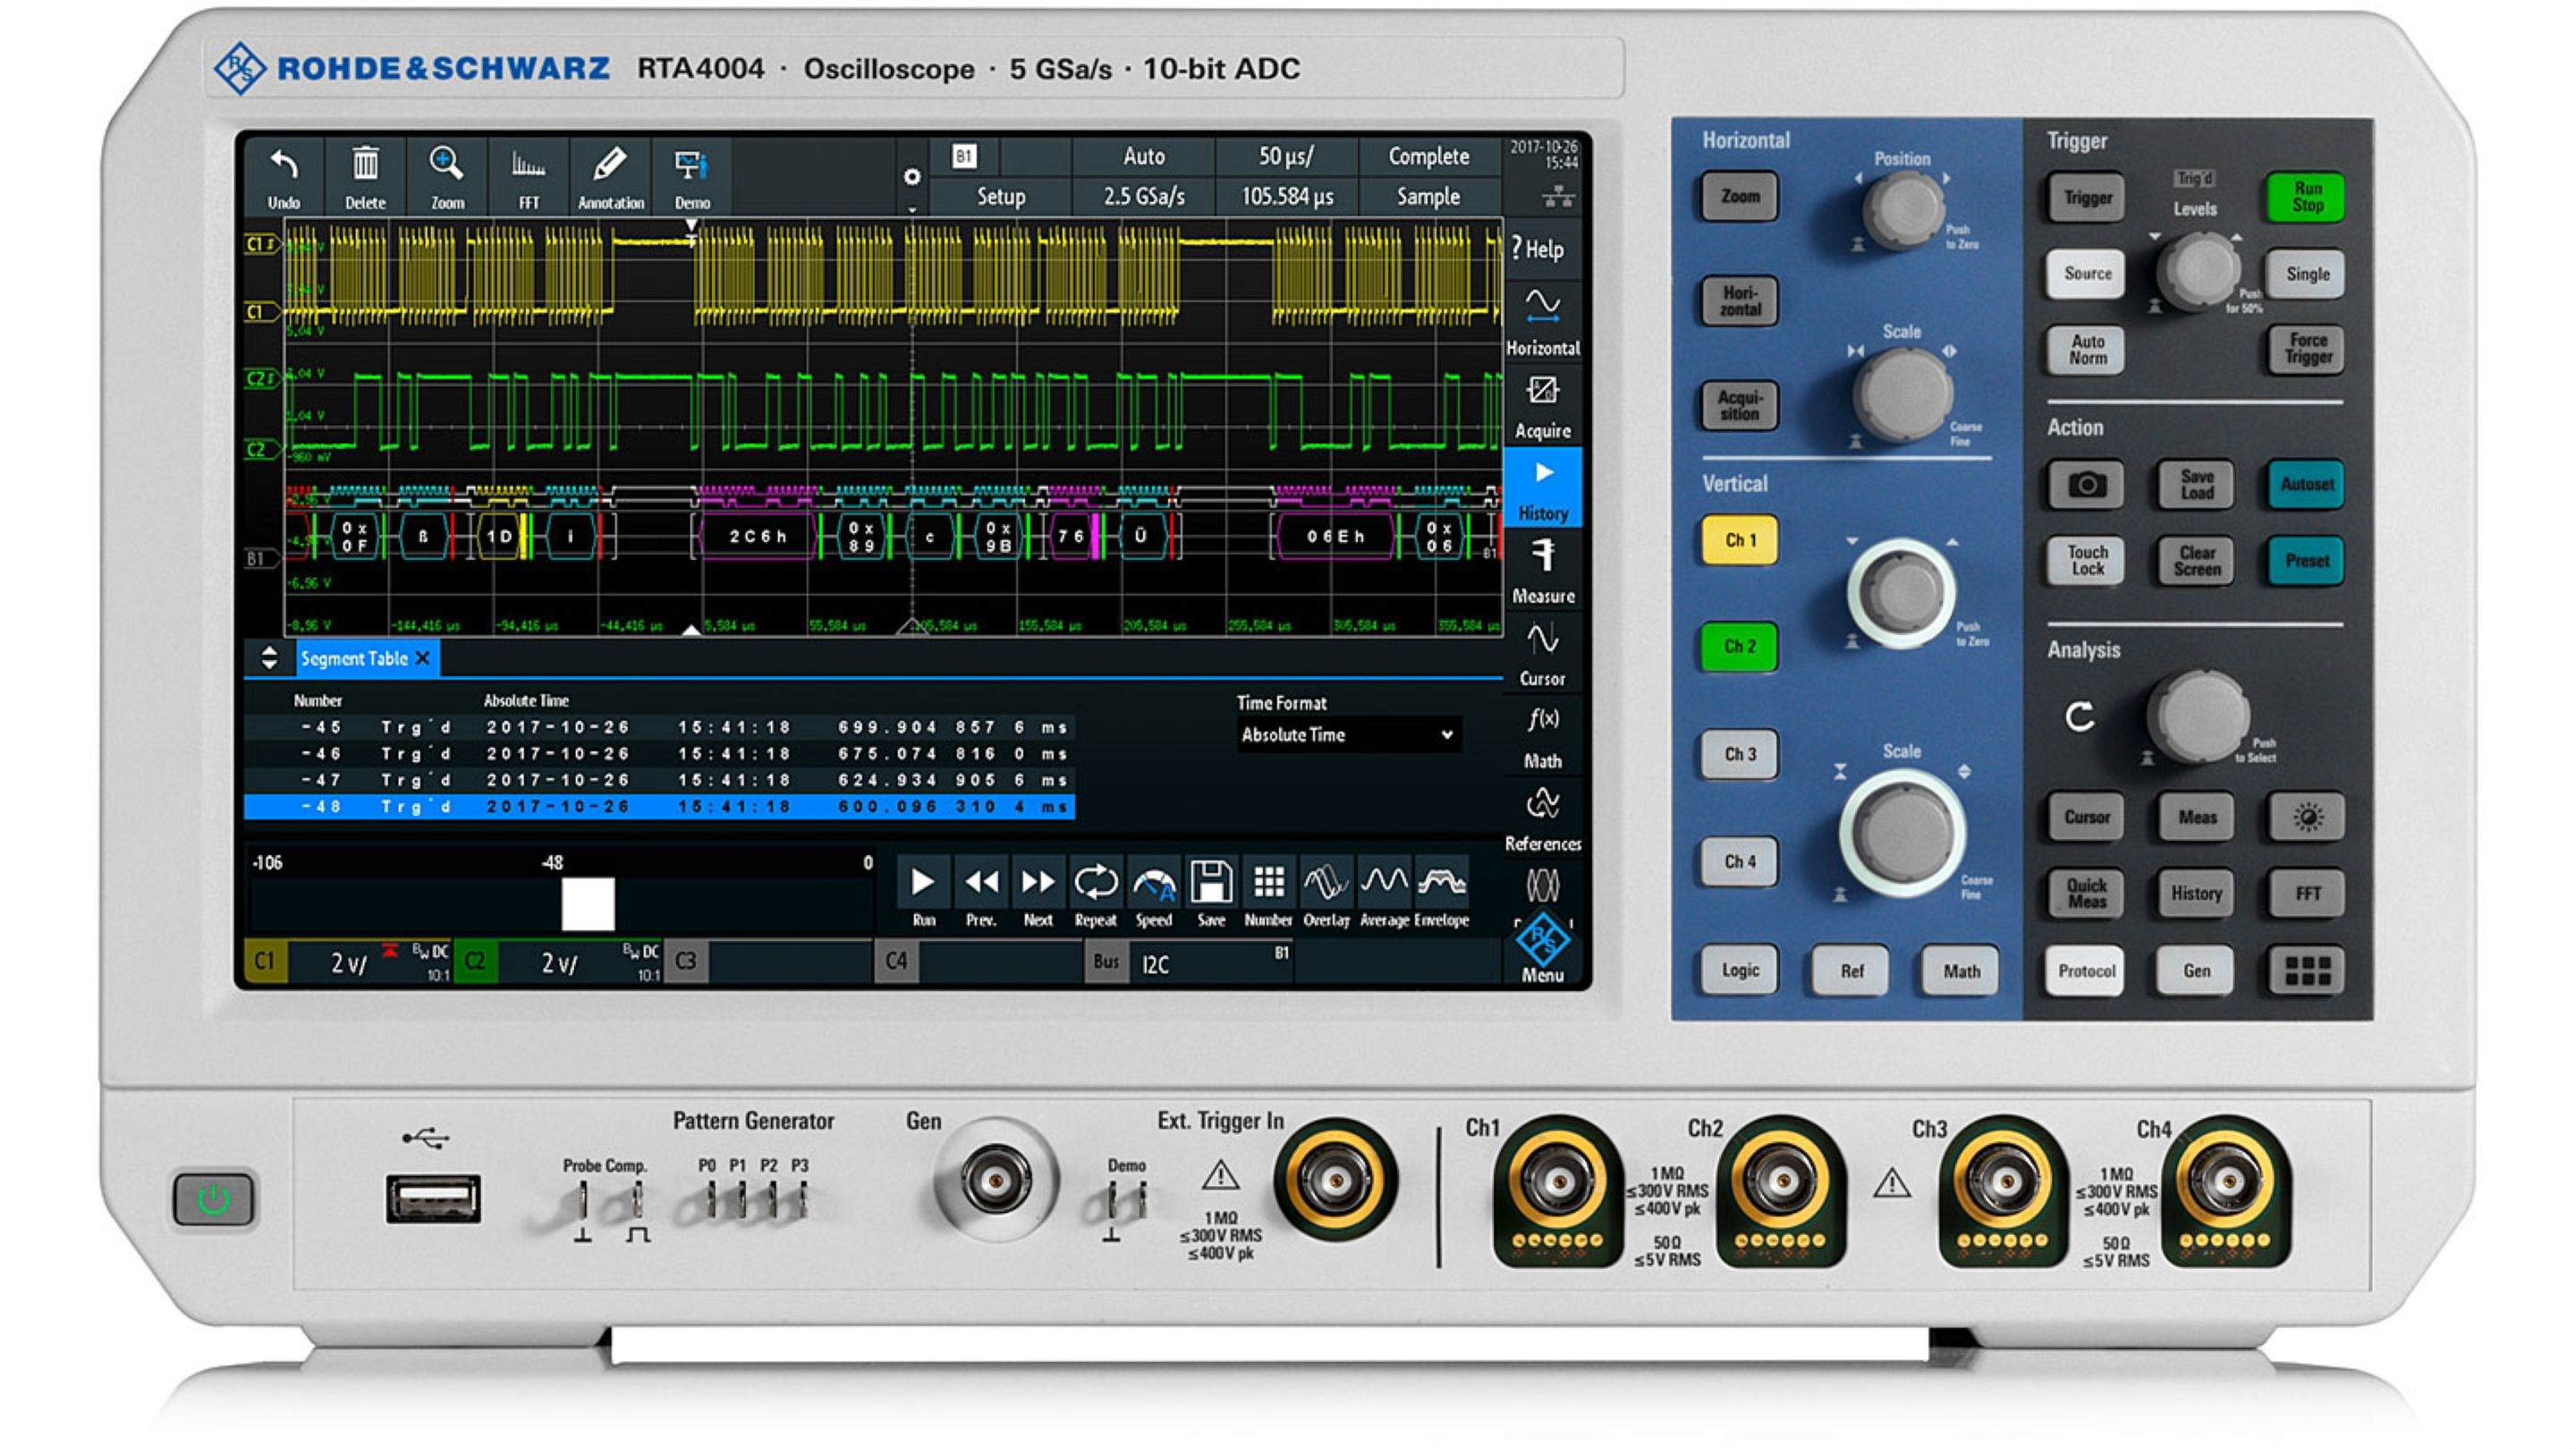
\includegraphics[height = 0.3 \textheight]{figures/rohde.jpg}
            \begin{figure}
                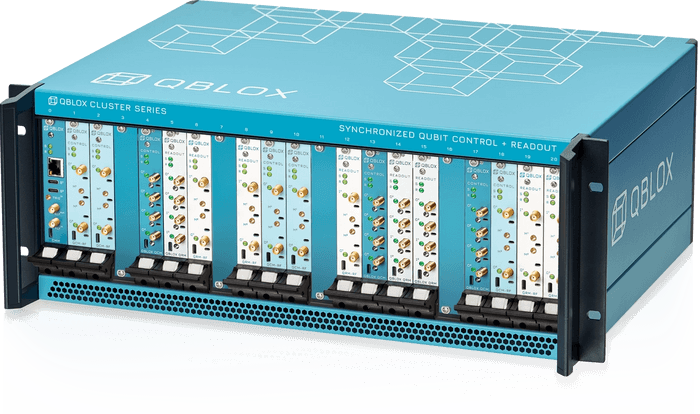
\includegraphics[height = 0.3 \textheight]{figures/qblox.png}
                % \caption{Qblox}
                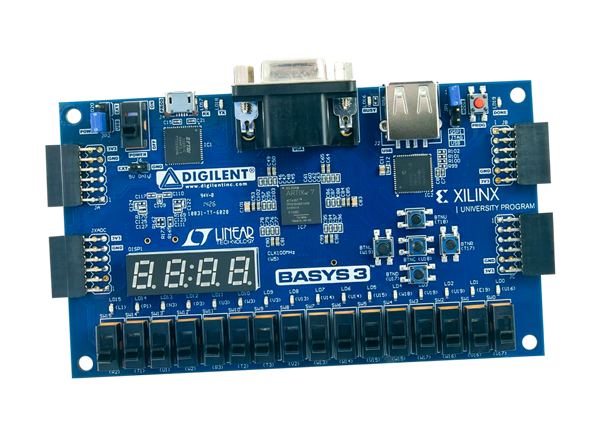
\includegraphics[height = 0.3 \textheight]{figures/fpga.png}
                % \caption{FPGA board}
            \end{figure}
            
        \end{column}
    \end{columns}
  
   We need a framework to control all these devices at the same time.
    
\end{frame}

\begin{frame}{Introducing Qibolab}
    \begin{columns}
        \begin{column}[]{0.5 \textwidth}
            \begin{figure}
                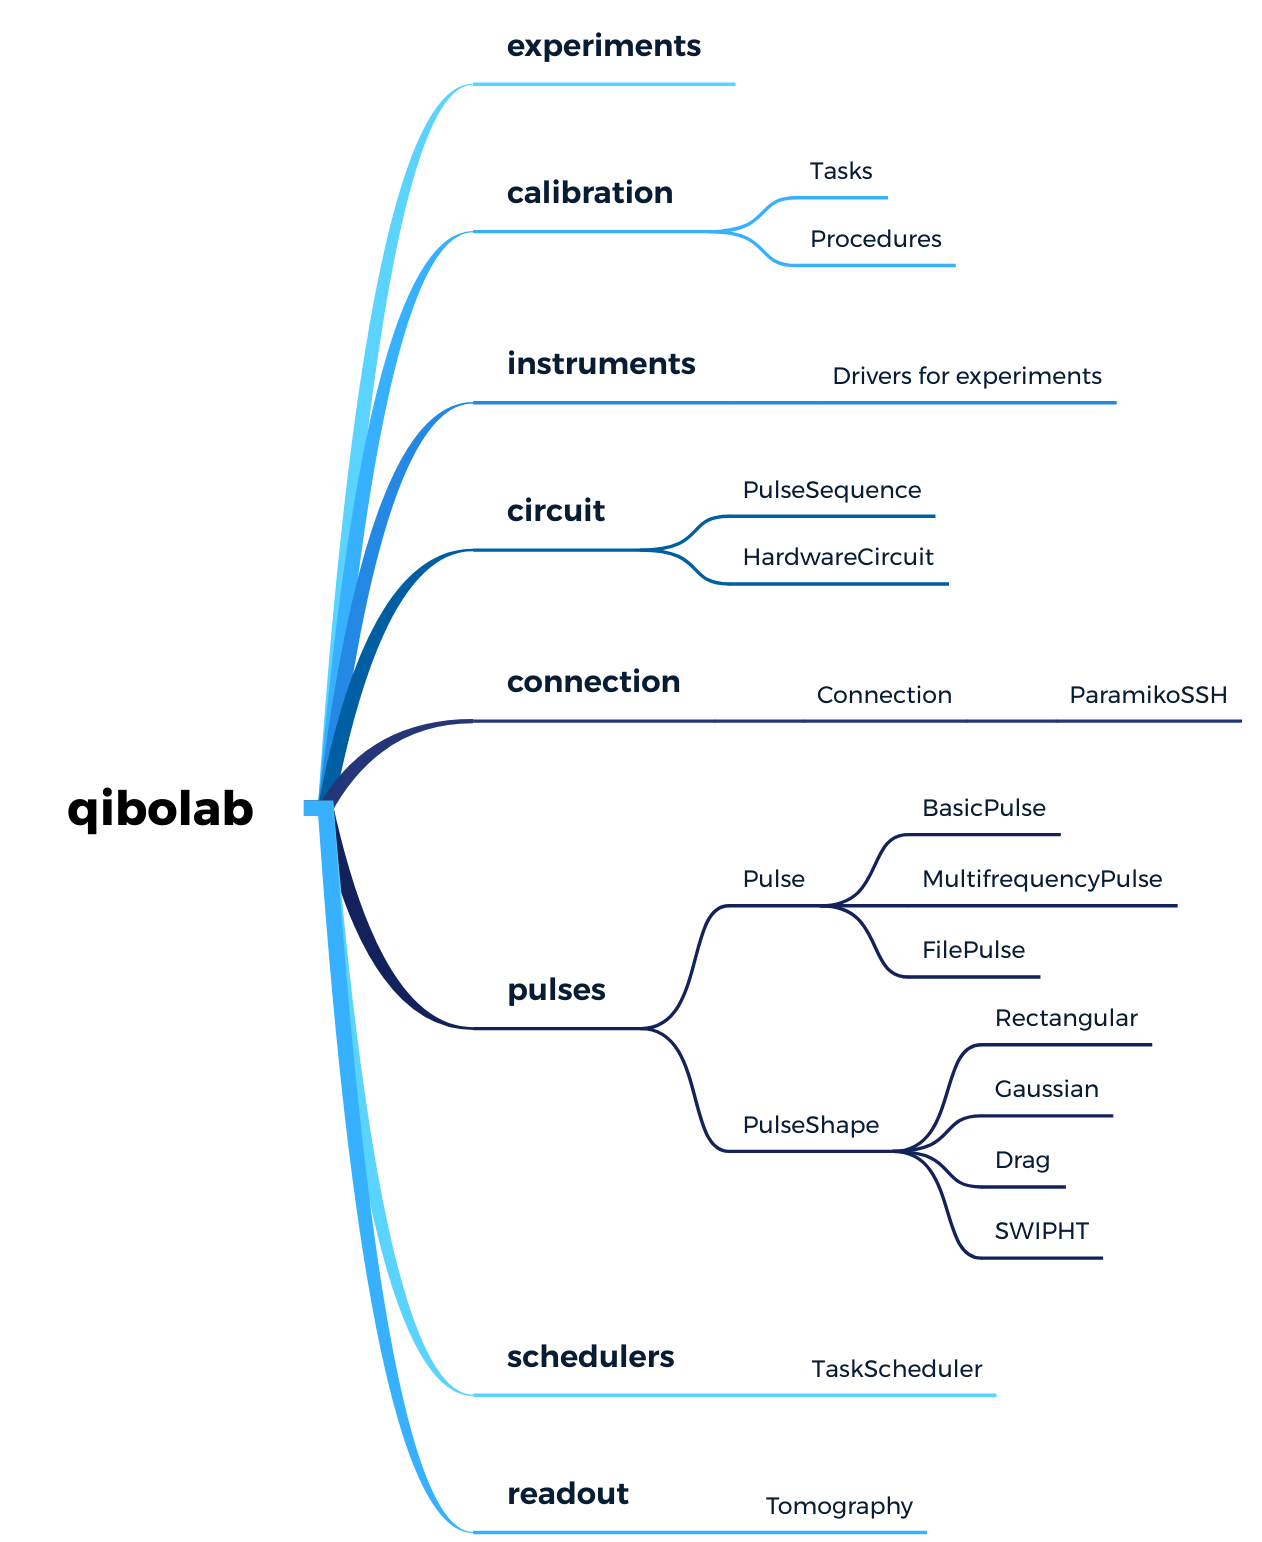
\includegraphics[height=0.8\textheight]{figures/qibolab.png}
            \end{figure}
            
        \end{column}

        \begin{column}[]{0.5 \textwidth}
            \begin{tcolorbox}[colframe=gray,title=Qibolab key features:]
                \begin{itemize}
                    \item Create \textbf{custom experimental drivers} for lab setup
                    \item Platform \textbf{agnostic} layout
                    \item Deploy \textbf{Qibo models} on quantum hardware easily
                \end{itemize}
                \end{tcolorbox}
        \end{column}
    \end{columns}
\end{frame}





\section{A reporting tool for calibration using Qibo}

\begin{frame}{Motivation}
    Suppose that we have assembled a quantum computer and we have a way
    to send pulses to the chip... are we done? {\color{red} \textbf{No} }

    We need to { \color{blue} characterize}, { \color{blue} validate} and { \color{blue} verificate} our qubits (QCVV):
    % \begin{columns}
    %     \begin{column}{0.5 \textwidth}
    %         \vspace{-2cm}
        %     \begin{itemize}
        %         \item[\faCaretSquareORight] Perform standard calibration routines:
        %         \begin{itemize}
        %             \item[\faWrench] Resonator and qubit spectroscopy
        %             \item[\faWrench] Rabi and Ramsey 
        %             \item[\faWrench] T1 and T2 determination
                
        %         \end{itemize}
        %         \item[\faCaretSquareORight] Perform quantum protocols to extract the fidelity:
        %         \begin{itemize}
        %             \item[\faWrench] Randomized Benchmarking
        %             \item[\faWrench] Gate Set Tomography
        %             \item[\faWrench] Cross-Entropy Benchmarking
        %         \end{itemize}
        %         \item[\faCaretSquareORight] Repeat the above steps periodically.
        %     \end{itemize}
        % \end{column}
        % \begin{column}{0.5 \textwidth}
            \begin{multicols*}{2}
                \begin{figure}
                    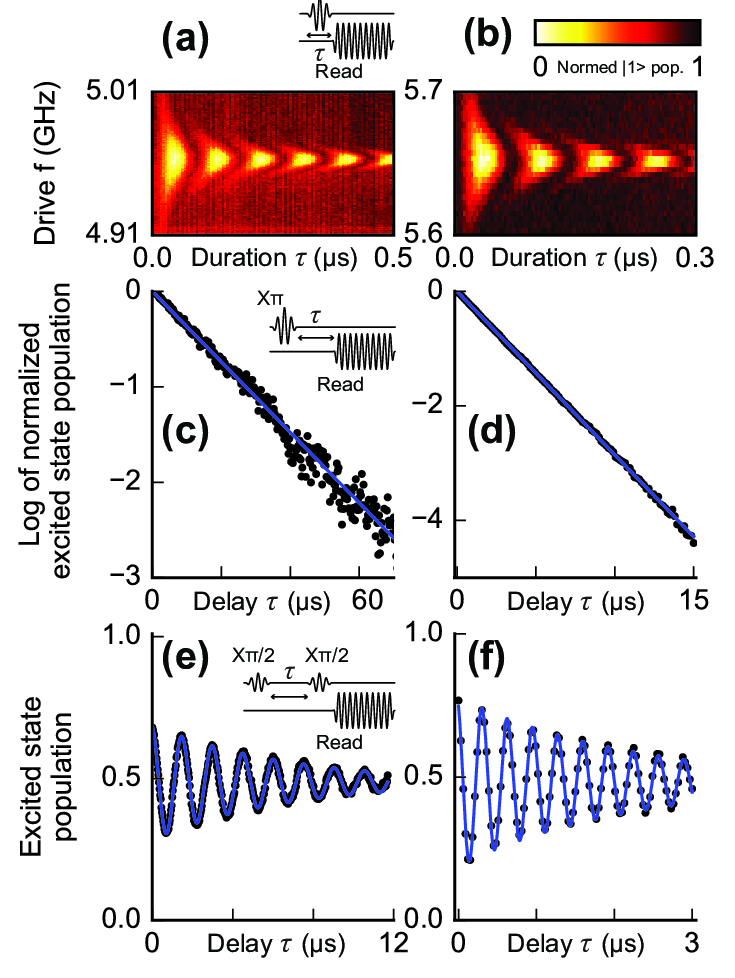
\includegraphics[height = 0.7 \textheight]{figures/characterization.png}
                \end{figure}

                \begin{figure}
                    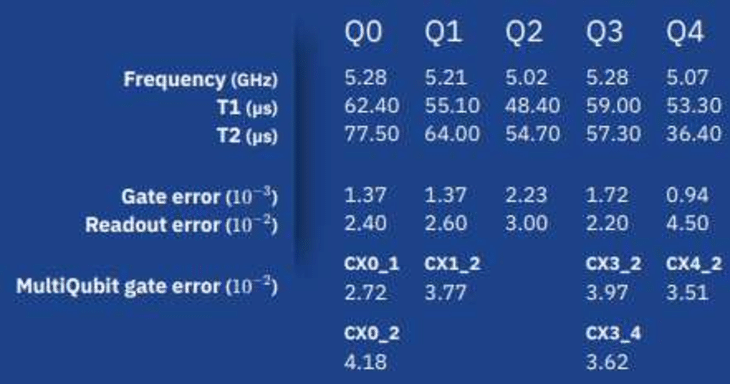
\includegraphics[width = 0.5 \textwidth]{figures/ibm.png}
                \end{figure}
            \end{multicols*}
            
            
    %     \end{column}
    % \end{columns}
    

\end{frame}

\begin{frame}{Single Qubit characterization}
    \begin{figure}
        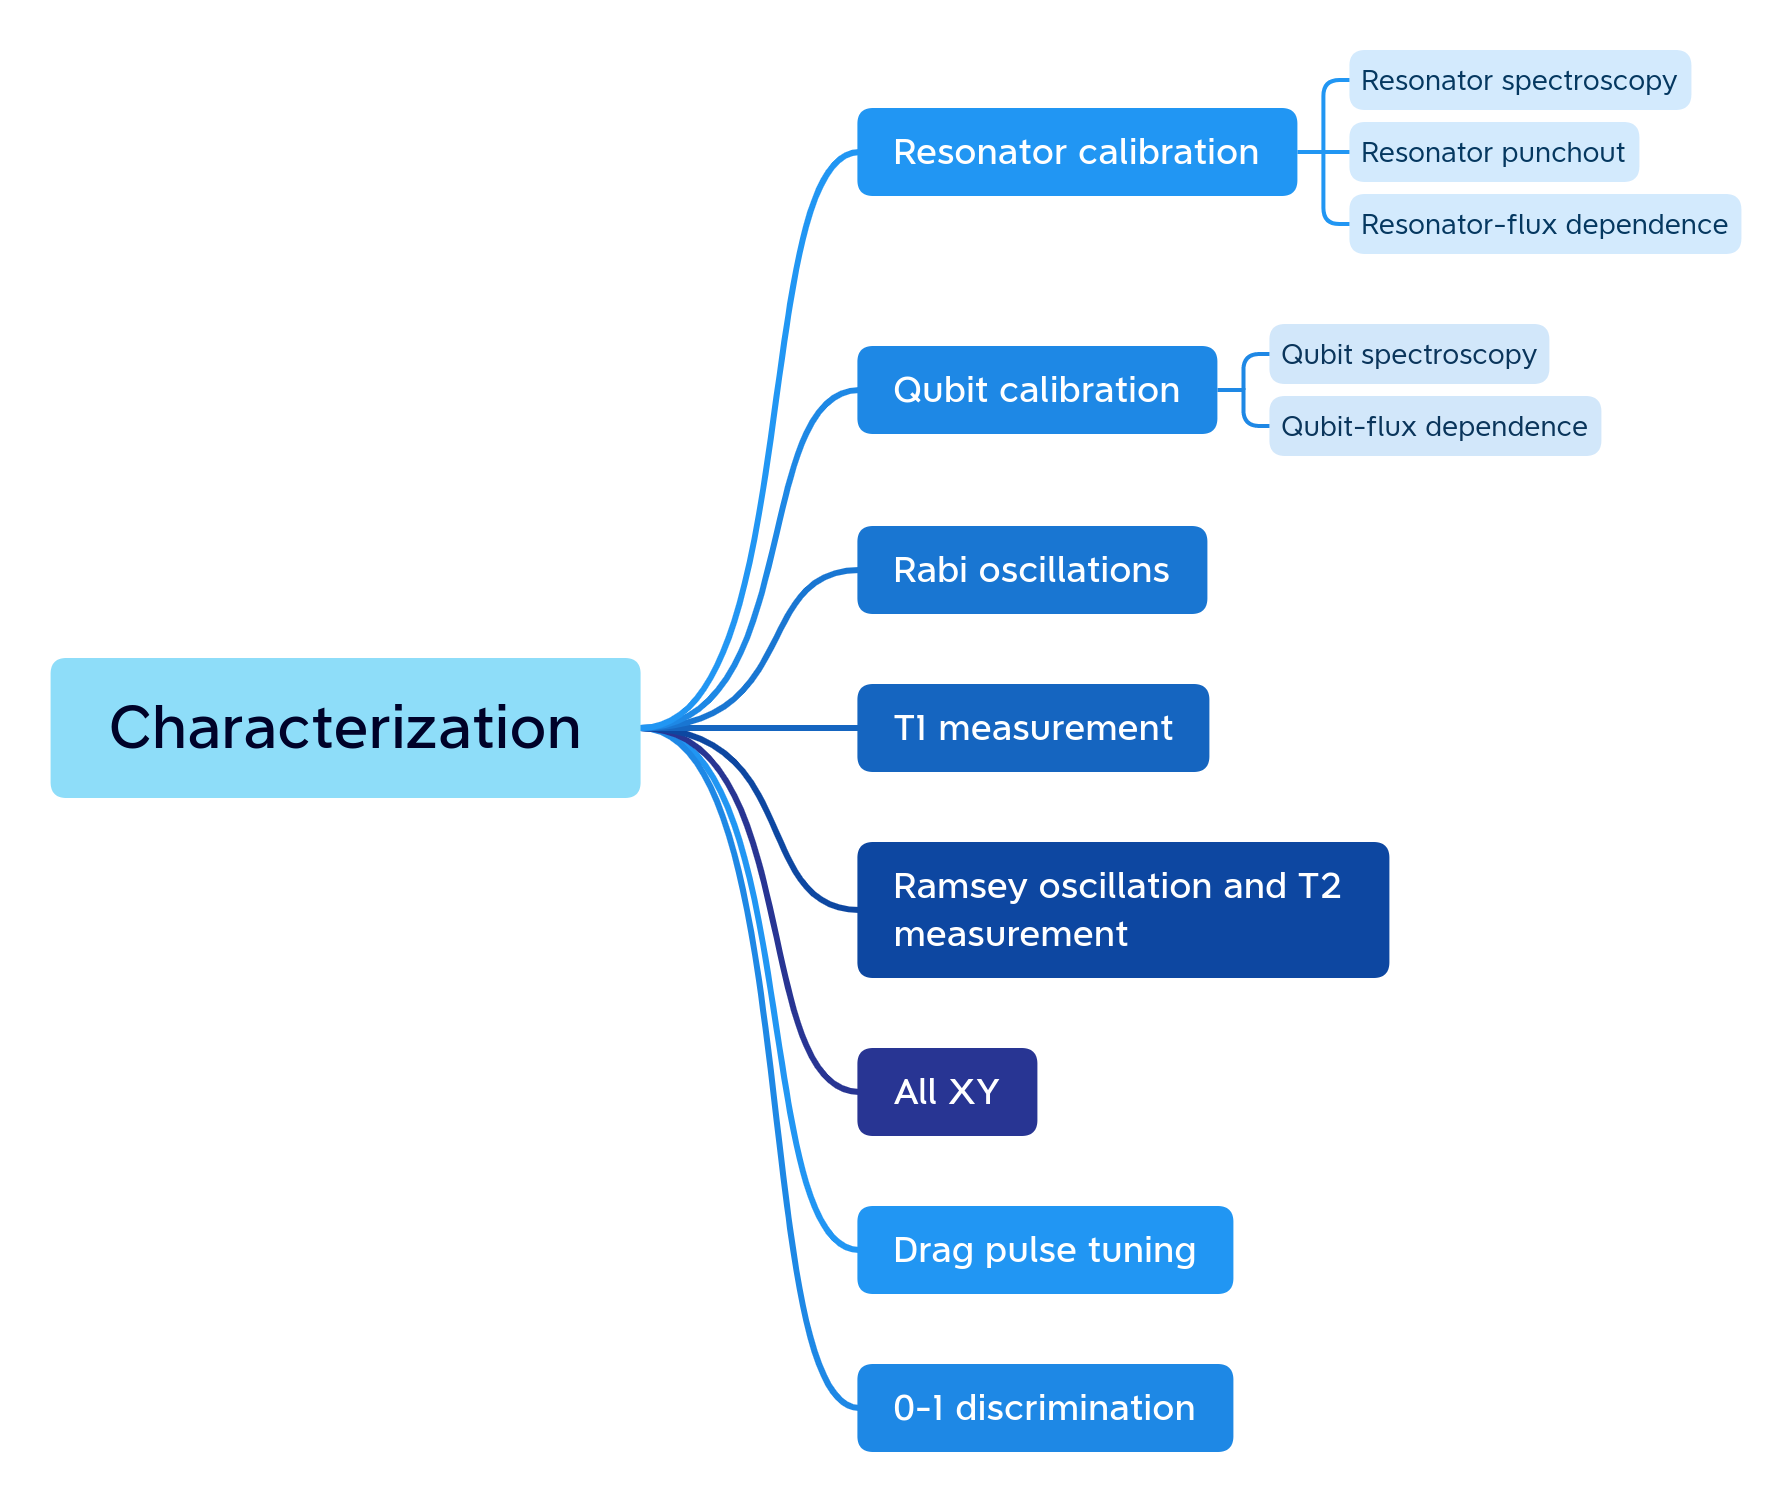
\includegraphics[width= 0.8 \textwidth]{figures/Characterization.png}
    \end{figure}
\end{frame}

\begin{frame}{Quantum benchmarking protocols}
    After characterizing our quantum hardware we need to compute the gates
    error behavior.

    In the current state-of-the-art this is computed using \textbf{Quantum
        benchmarking protocols}.
    \begin{figure}
        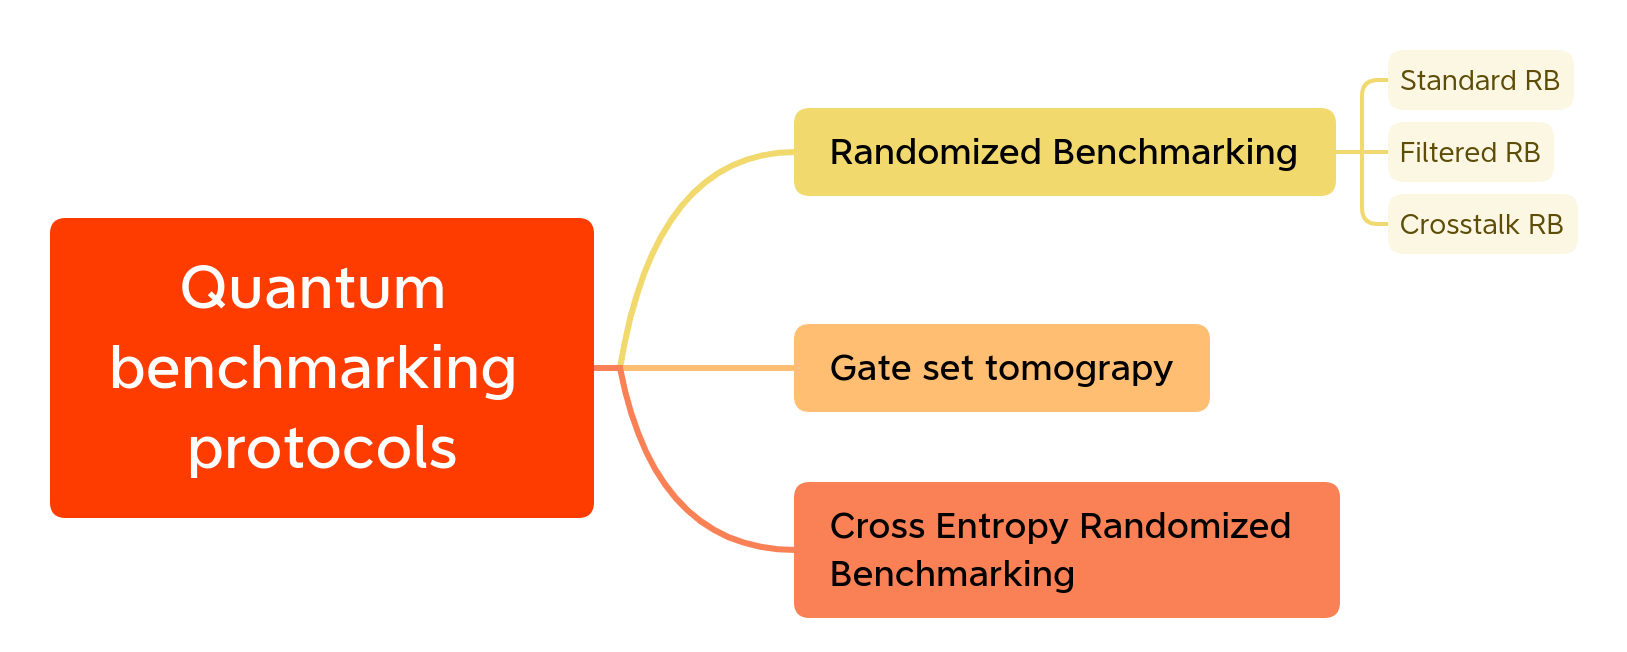
\includegraphics[width= 0.8 \textwidth]{figures/Quantum protocols.png}
    \end{figure}

    In Qibocal we are currently developing a suite for the execution of the
    latest QBP available.
\end{frame}

\begin{frame}{Motivation}
    We are developing a new tool called {\color{blue} \textbf{Qibocal}} to perform qubits calibration in Qibo using Qibolab as the main driver.
    
    The main features that we are implemented are the following:


    \begin{multicols*}{2}
        \begin{itemize}
            \item[\faCaretSquareORight] Platform agnostic approach
            \item[\faCaretSquareORight] Launch calibration routines easily
            \item[\faCaretSquareORight] Live-plotting tools
            \item[\faCaretSquareORight] Live-fitting tools
            \item[\faCaretSquareORight] Save and share your data
            \item[\faCaretSquareORight] Autocalibration
        \end{itemize}
    \end{multicols*}
\end{frame}

\begin{frame}{Qibocal: implementation}
    \begin{figure}
        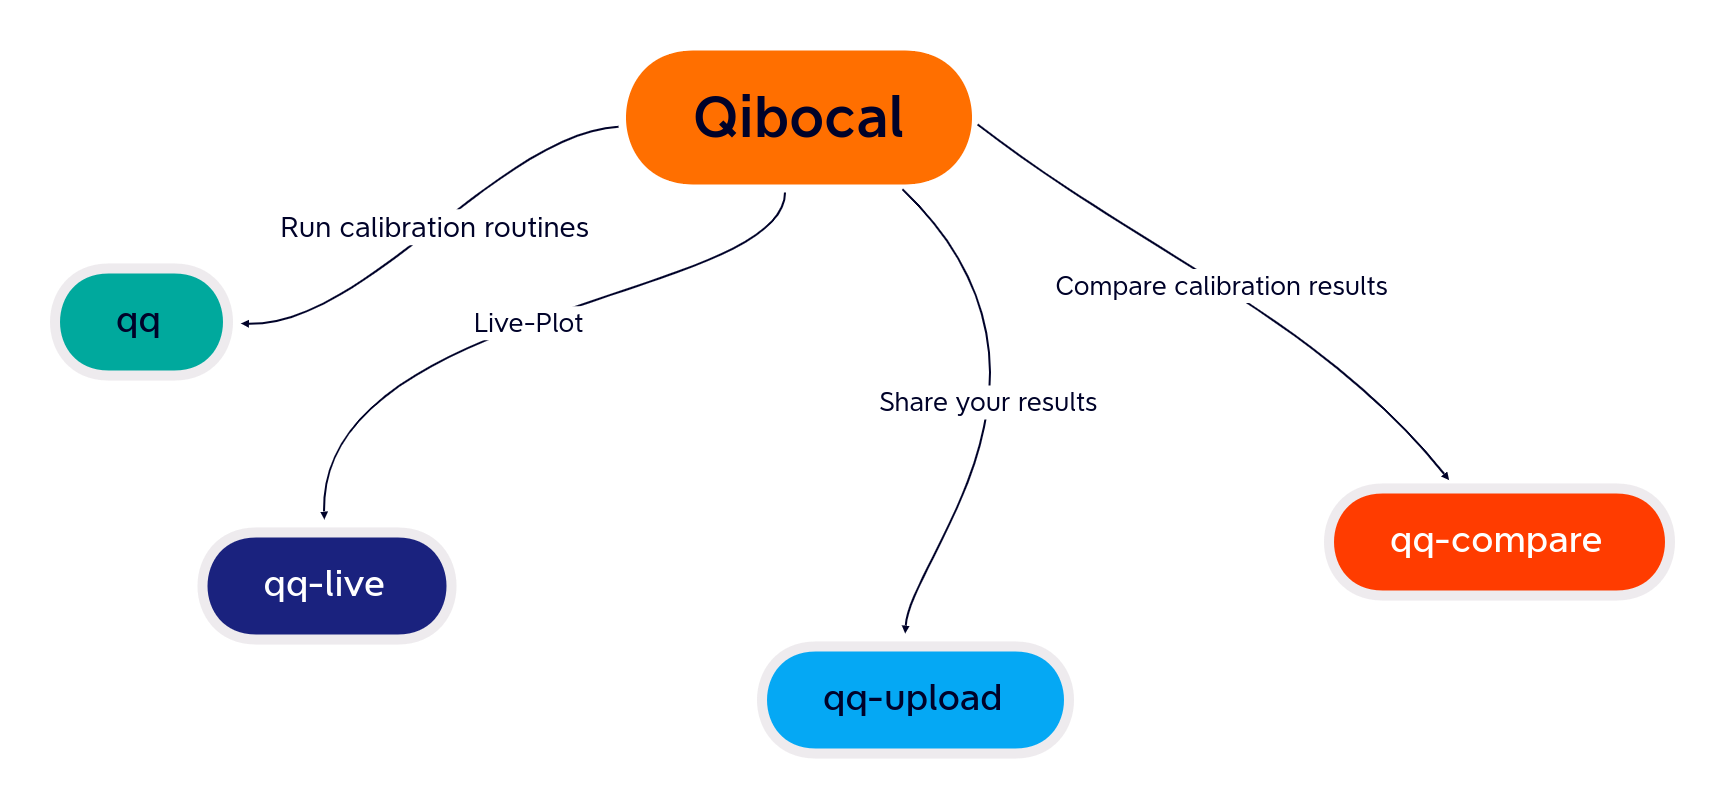
\includegraphics[width= \textwidth]{figures/Qibocal.png}
    \end{figure}
\end{frame}



\begin{frame}{How to use \texttt{qq}}
    To run a specific set of calibration it is sufficient to write a runcard:
    \begin{multicols*}{2}
        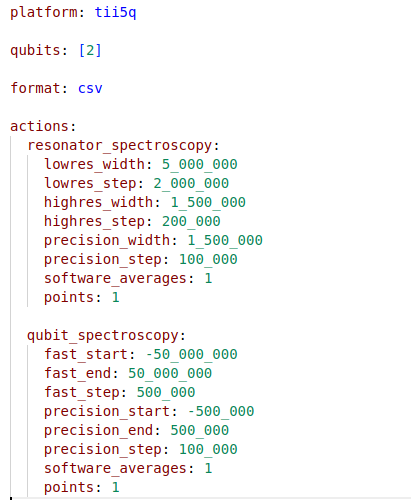
\includegraphics[width= 0.5 \textwidth]{figures/runcard.png}
        You can execute the following runcard by typing:
        \begin{center}
            \texttt{qq} \texttt{<runcard.yaml>} 
        \end{center}

    \texttt{qq} will take care of:
    \begin{itemize}
        \item connecting to the platform
        \item executing the routines listed under actions
        \item generating an update runcard for the platform
        \item generating a web report containing the results
    \end{itemize}
    \end{multicols*}
    \
\end{frame}

\begin{frame}{How to use \texttt{qq-live}}
    Using \texttt{qq-live} it is possible to visualize the results during (after) the execution
    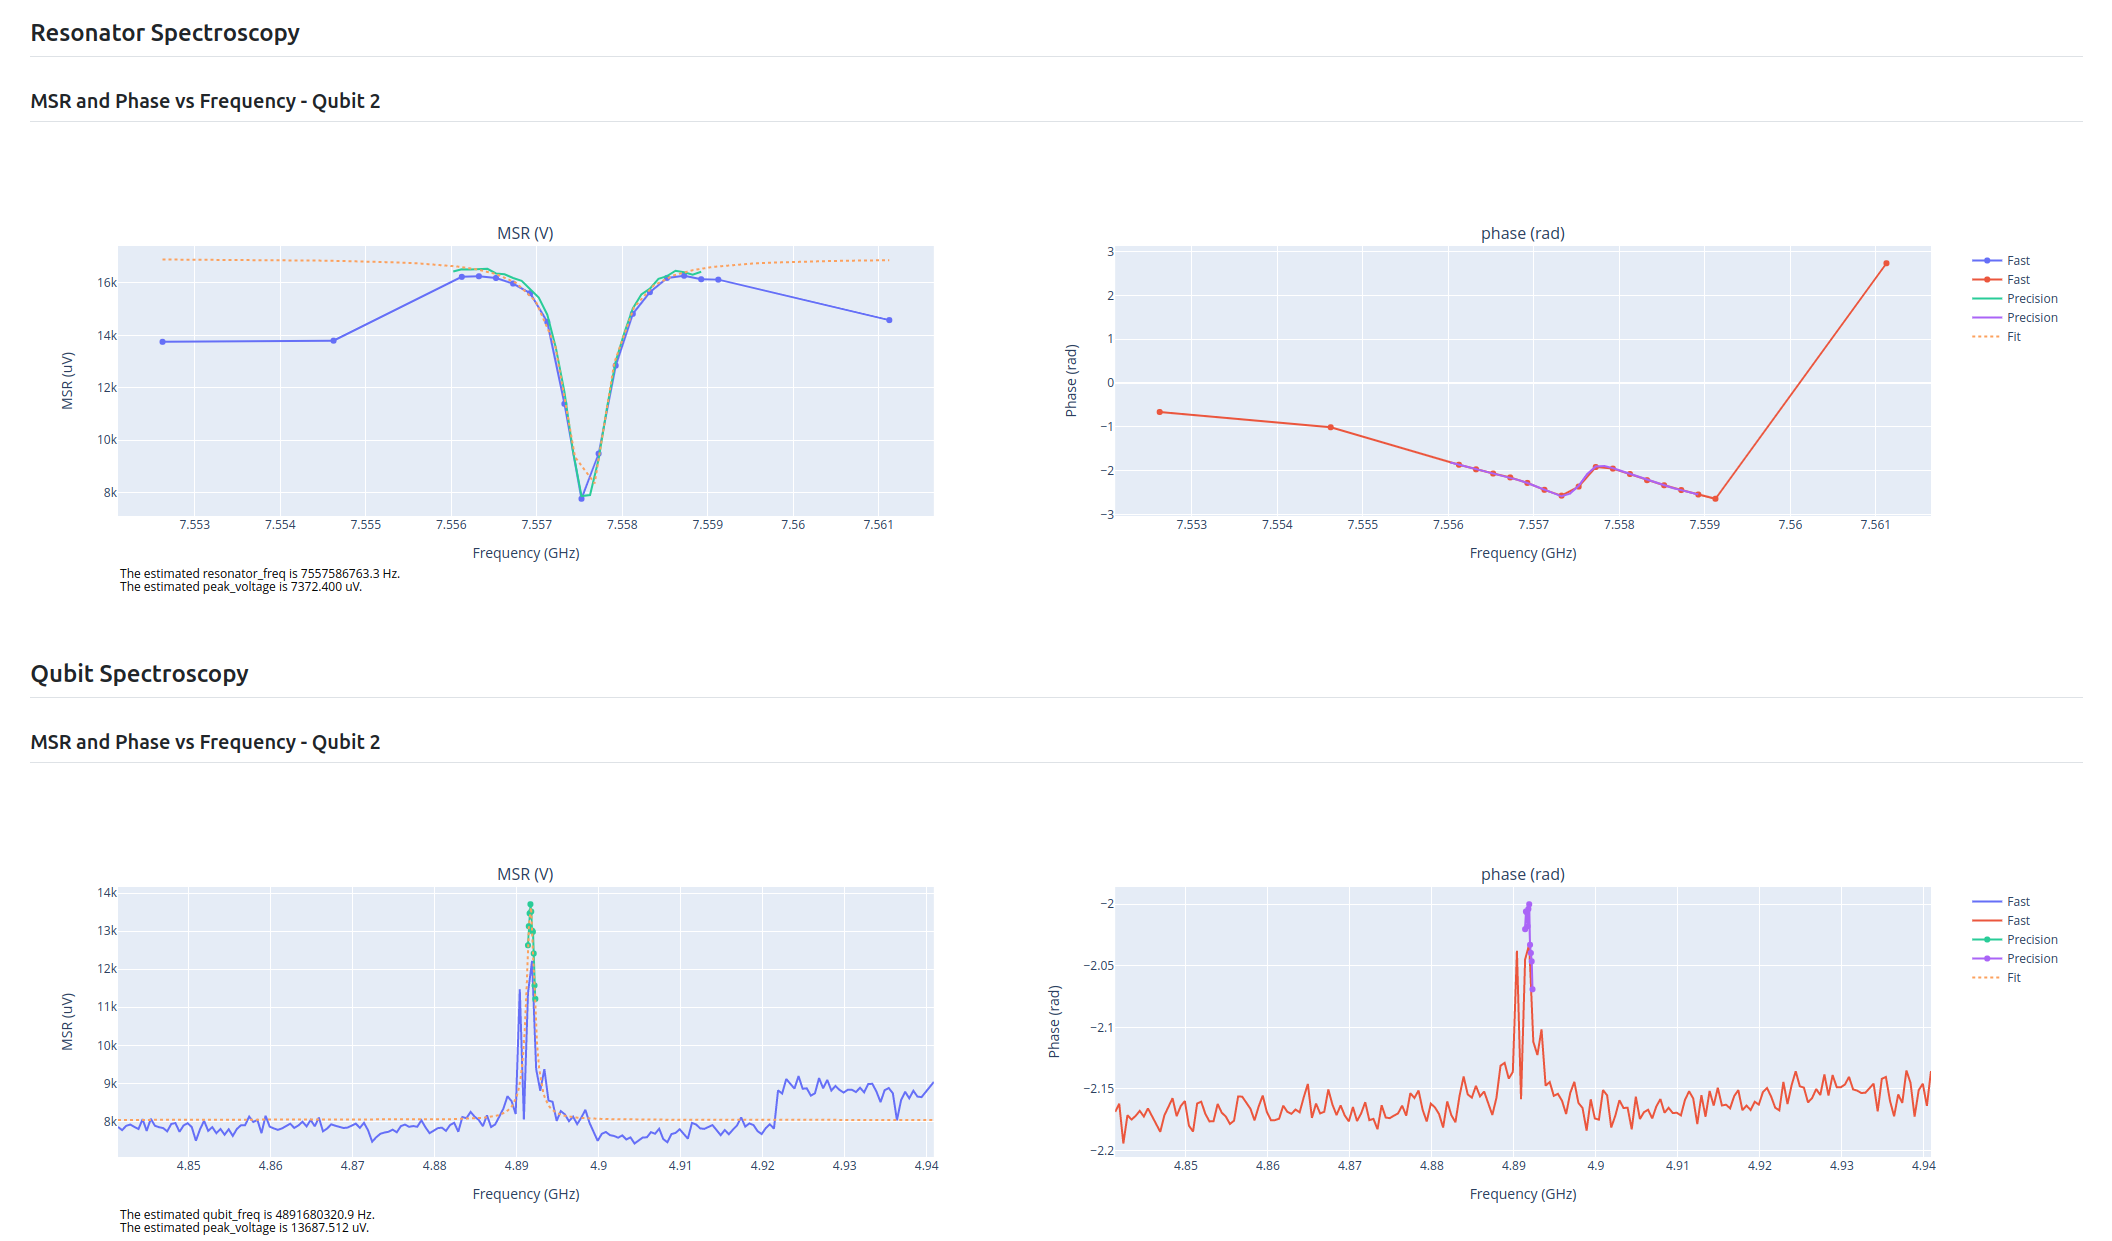
\includegraphics[width=\textwidth]{figures/qq-live.png}
\end{frame}

\begin{frame}{How to use \texttt{qq-upload}}
    
    You can share your results by uploading the report generated by \texttt{qq} using \texttt{qq-upload}
    \vspace{0.3cm}
    
    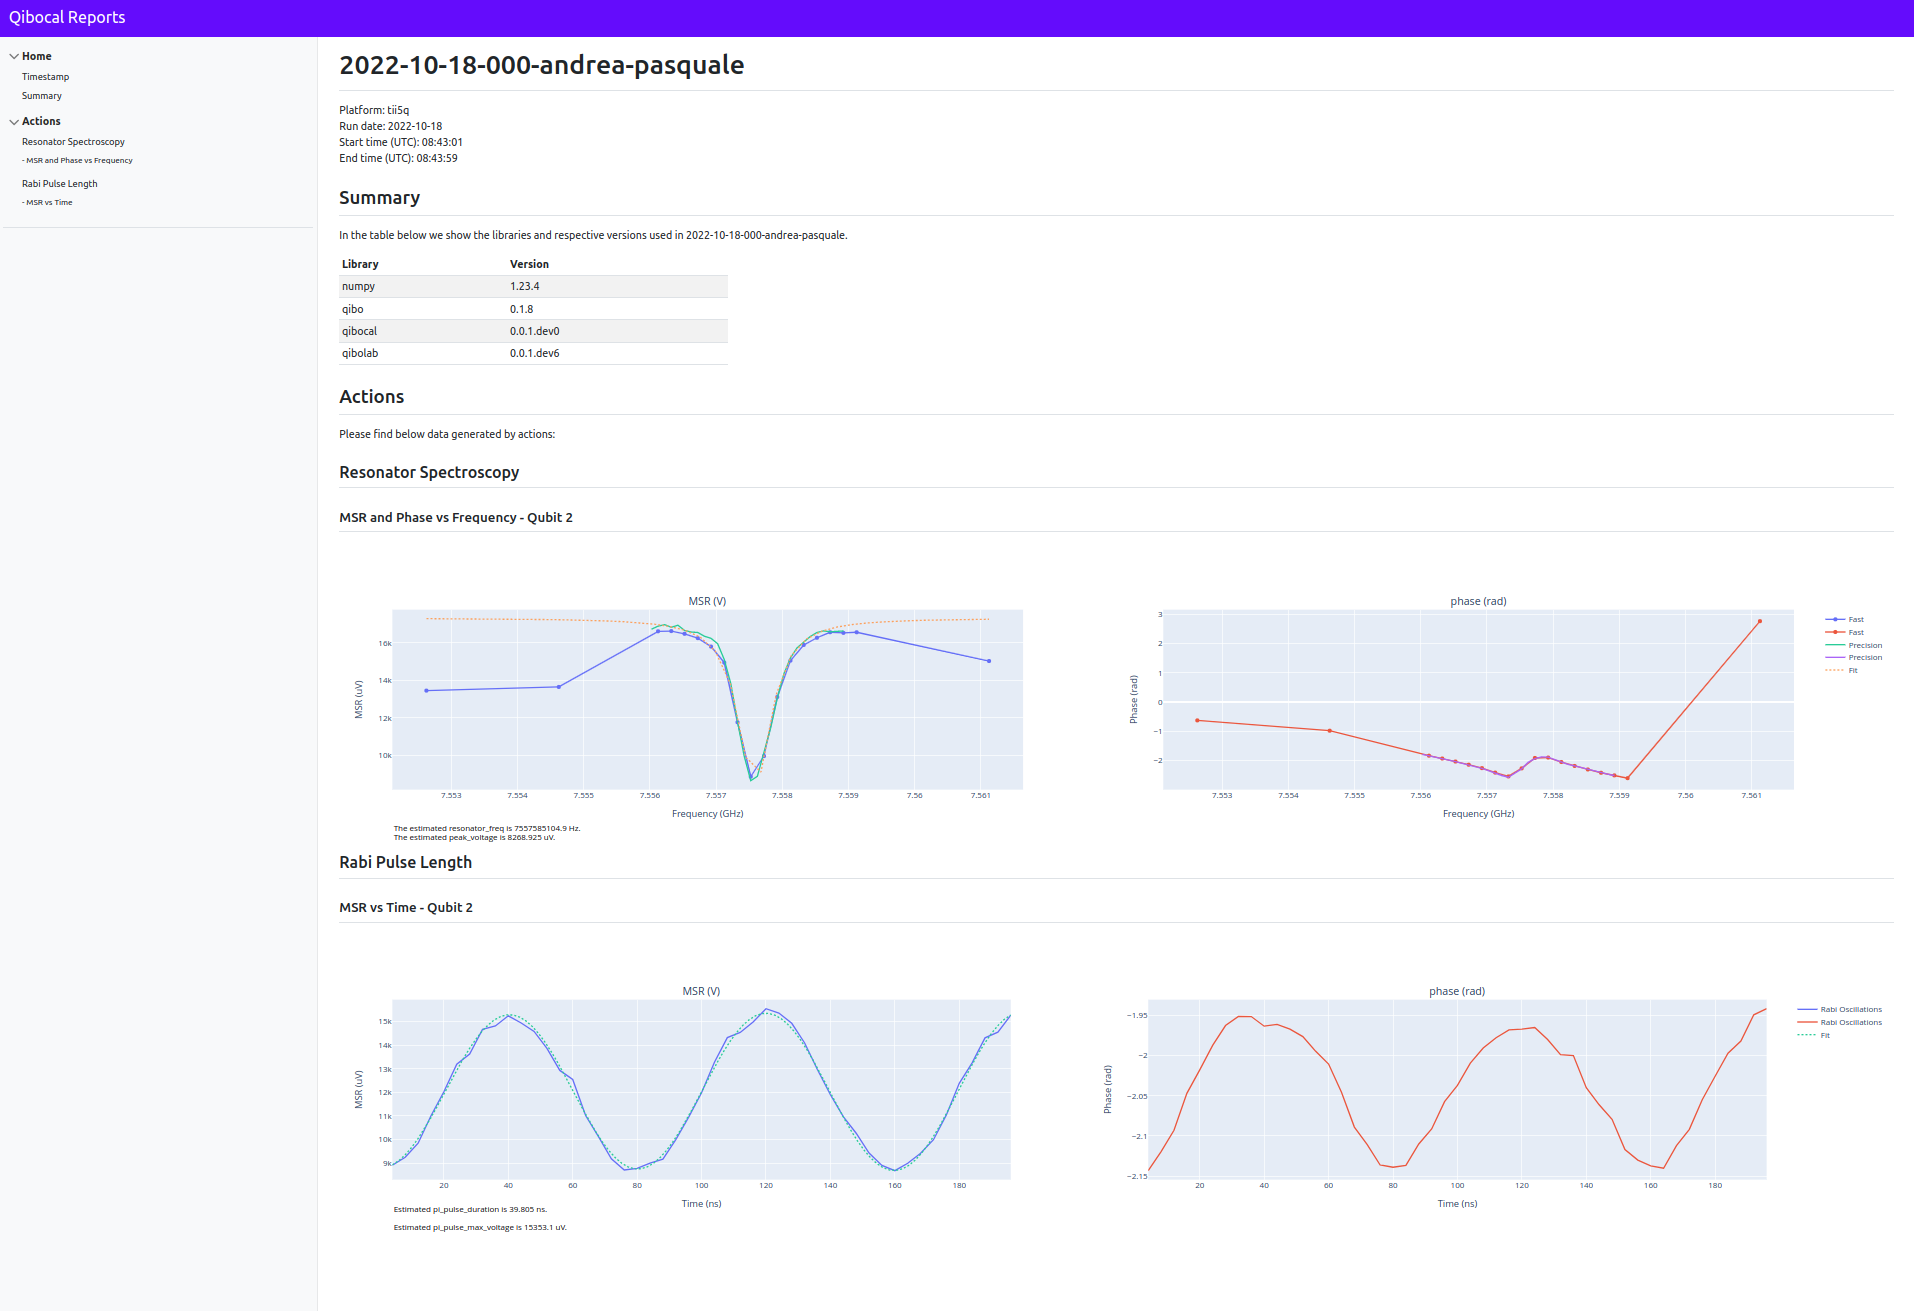
\includegraphics[width=\textwidth]{figures/upload.png}
\end{frame}


\section{Applications}

\begin{frame}{Applications}
    What can we achieve using Qibo + Qibolab + Qibocal?

    Successfully performed a \textbf{gradient descent on a
    QPU} with one qubit using the Parameter Shift Rule algorithm.

    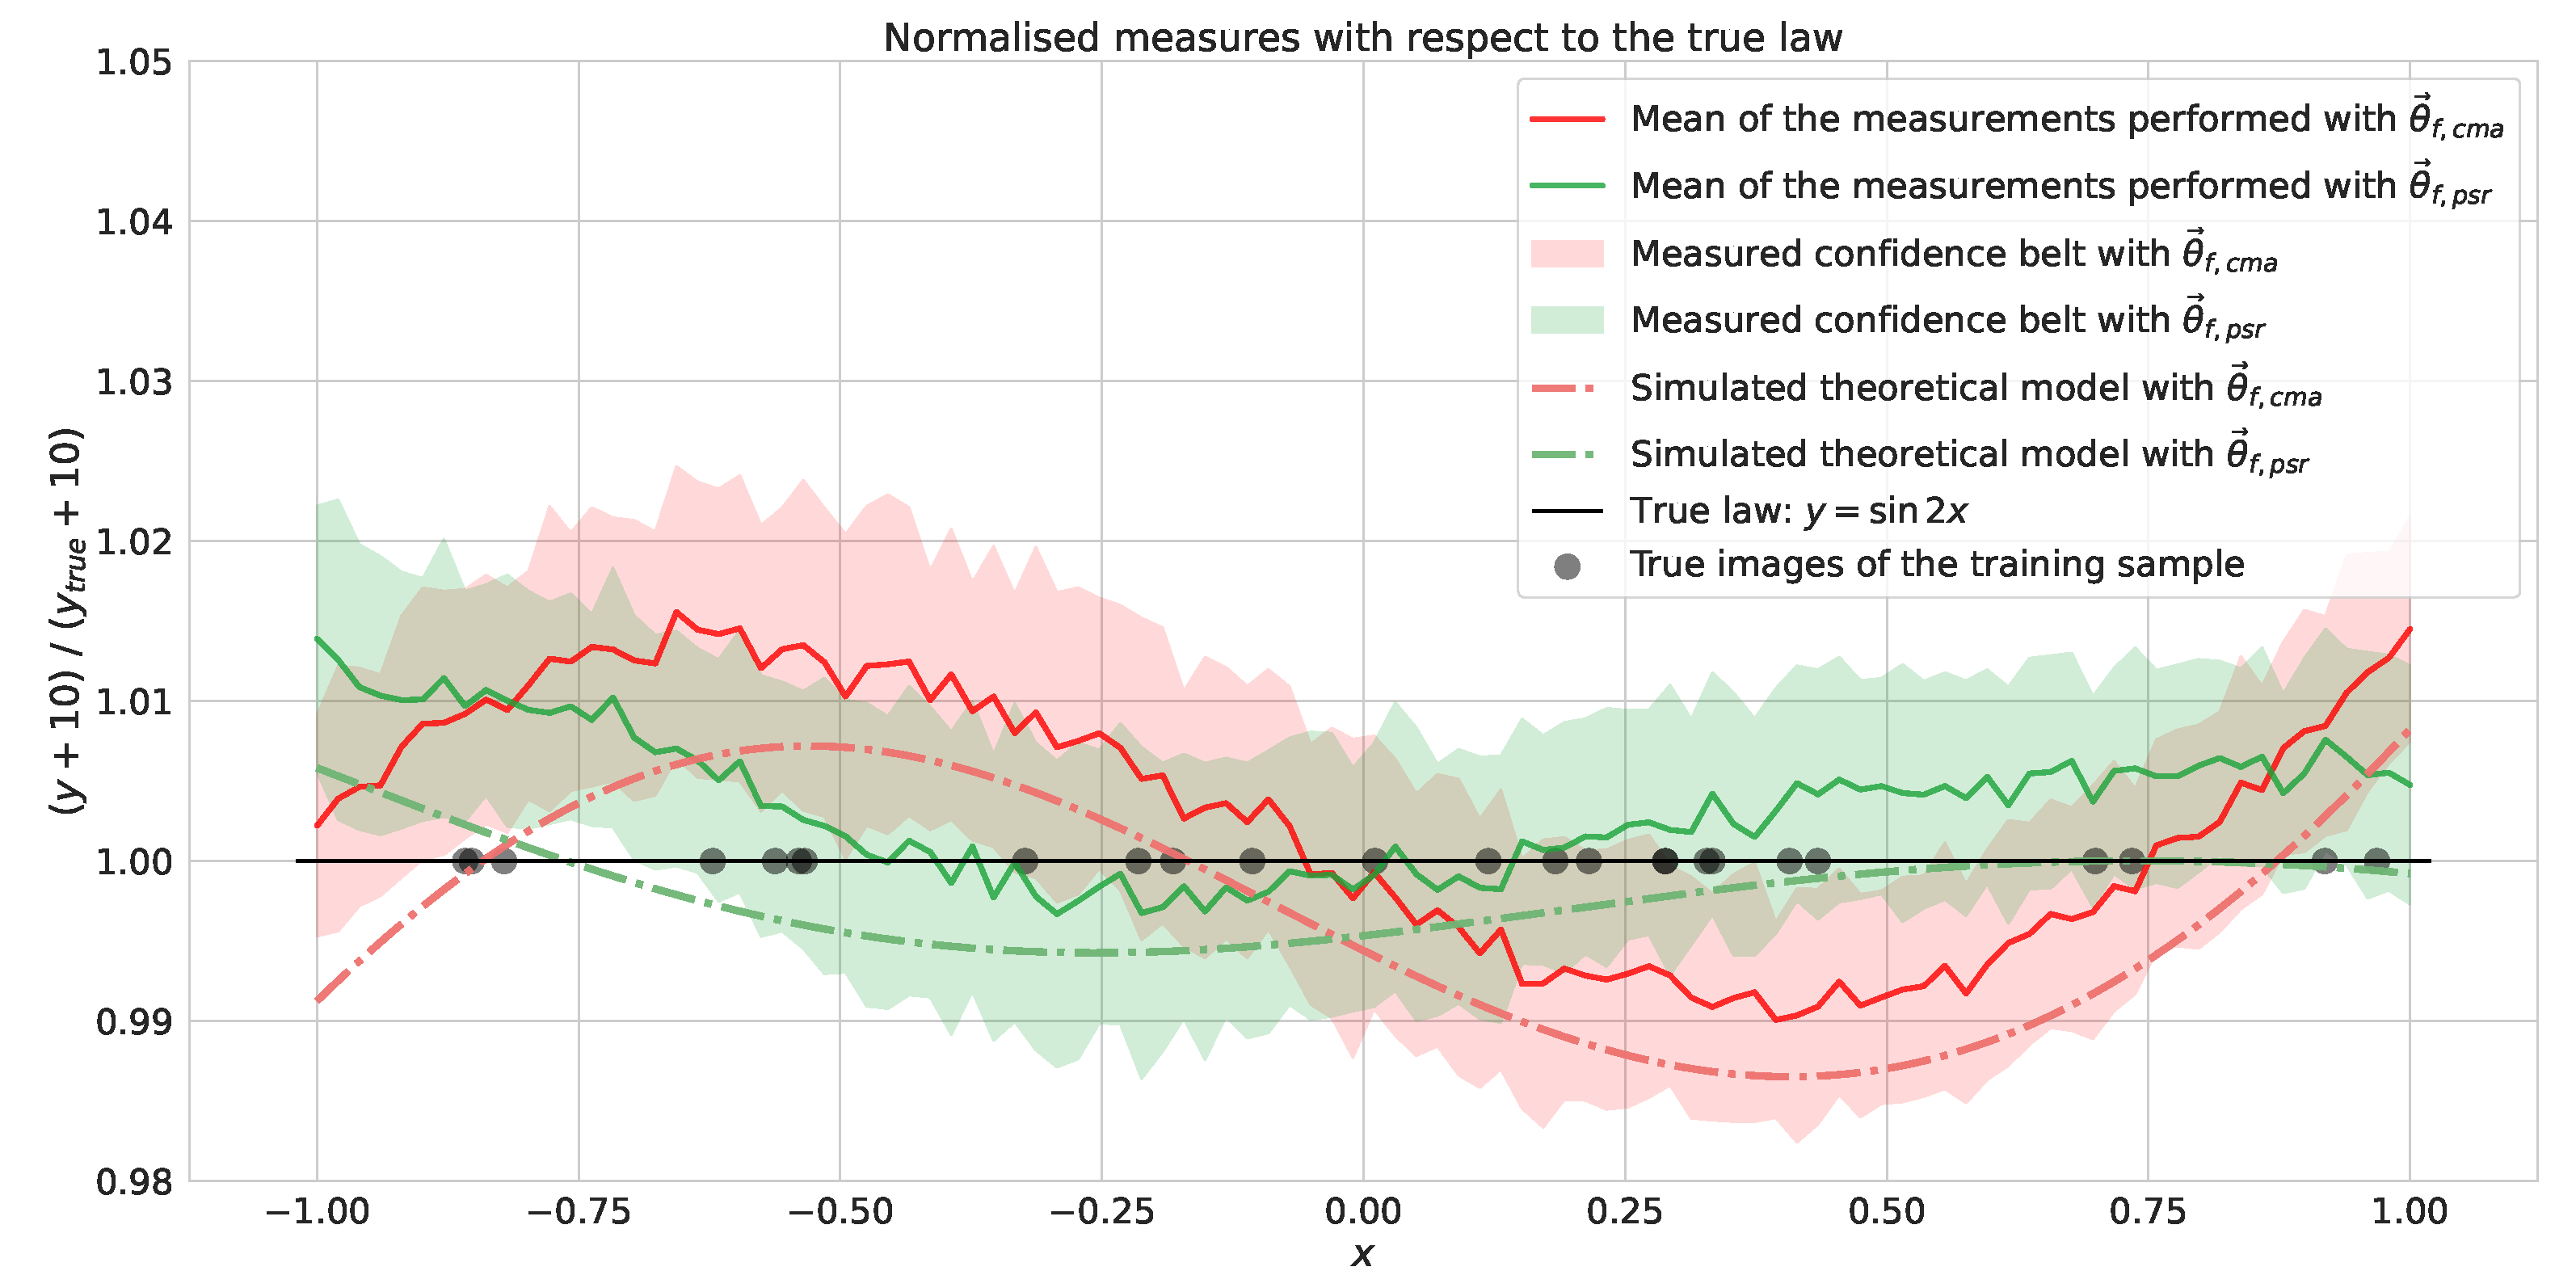
\includegraphics[width=\textwidth]{figures/normed_results.pdf}


    \url{https://arxiv.org/pdf/2210.10787.pdf}
\end{frame}


\begin{frame}{Outlook}
    Qibo is growing to accommodate different tasks:
    \begin{wrapfigure}{r}{0.25\textwidth}
        
\includegraphics[width=0.9\linewidth]{figures/qibo_logo.png} 
        \end{wrapfigure}
    \begin{itemize}
        \item[ \color{teal} \faCheck] High performance quantum simulation: {\color{blue} qibojit}
        \item[ \color{teal}\faCheck] Hardware control: {\color{red} qibolab}
        \item[ \color{teal} \faCheck] Hardware calibration: { \color{teal} \textbf{qibocal} }
    \end{itemize}

    What makes Qibo different from other libraries:
    \begin{itemize}
        \item[ \faPlus] Public available as an open source project.
        \item[ \faPlus] Modular layout design with possibility of adding
        \begin{itemize}
            \item a new backend for simulation
            \item a new platform for hardware control
        \end{itemize}
        \item[ \faPlus] Community driven effort
    \end{itemize}

    \url{https://github.com/qiboteam/qibo}

    \url{https://github.com/qiboteam/qibocal}
    
    \url{https://github.com/qiboteam/qibolab}
\end{frame}


\section{Thanks for listening!}

\section{Backup Slides}



% \begin{frame}
%     \includemovie{3cm}{3cm}{figures/puv1Q.gif}
% \end{frame}

\section{How can we implement physical qubits?}

\begin{frame}{Quantum technologies}
    \begin{figure}
        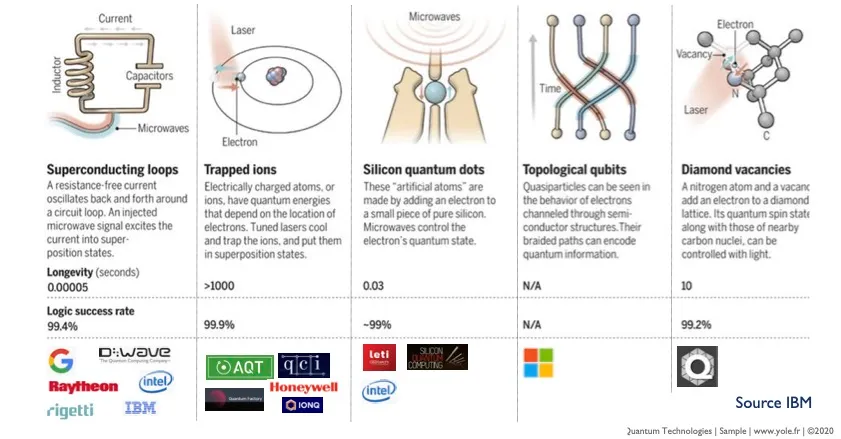
\includegraphics[width=\textwidth]{figures/quantum_technologies.png}
    \end{figure}
\end{frame}

\begin{frame}{How to use qibolab?}
    \begin{figure}
        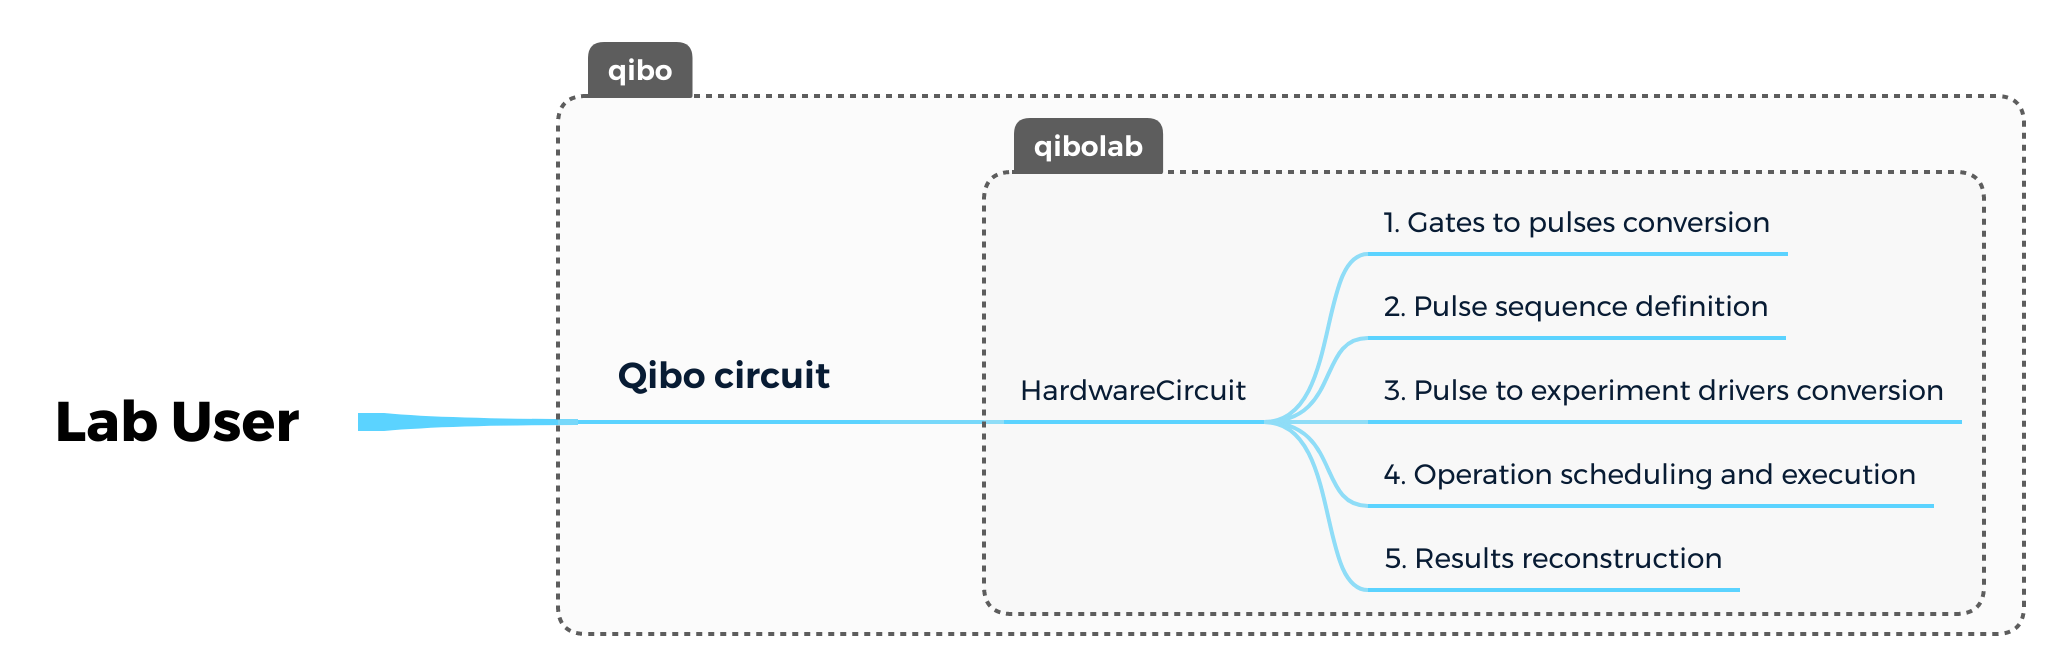
\includegraphics[width=\textwidth]{figures/hardwarecircuit.png}
    \end{figure}

    \begin{columns}
        \begin{column}{0.5 \textwidth}
            \begin{figure}
                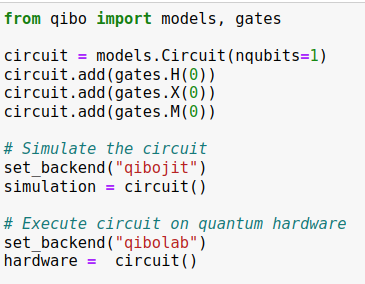
\includegraphics[width = \columnwidth]{figures/qibo__circuit.png}
            \end{figure}
        \end{column}
        \begin{column}{0.5 \textwidth}
            \begin{itemize}
                \item A single object to execute both on hardware and simulation
                \item Job scheduling to access the hardware using slurm
            \end{itemize}
            \centering
            
\includegraphics[height=2cm]{figures/Slurm_logo.svg.png}
        \end{column}
    \end{columns}

\end{frame}



\end{document}